\section{Simulating Compliant Humanoid Robots}
Simulation techniques for modern robot hardware could provide invaluable tools for design, research, and development for robot controllers.
For this reason, numerous efforts have been spent in developing robot simulators in the past two decades (\cite{DBLP:journals/corr/IvaldiPN14}), and more in general, in developing the large ecosystem that make simulating possible and convenient, from ever more fast and accurate dynamic solver libraries, to graphical editors for robotic systems and environments, planner libraries and visualization tools.

%%%%%%%%%%%% TITLE
\subsection{Simulators as Abstractions to the Physical Hardware:\\YARP Plugins for the Gazebo Simulator}

In the past years, robotics researchers have been developing several robotics frameworks, or middleware libraries, such as OpenRDK (\cite{cace08rdk}), YARP (\cite{Metta:YARP:2006}) or ROS (\cite{ROS}) in order to ease the creation of generic applications for robots and encourage code reuse. Some of these frameworks even enforce a component system \todo{cite orocos} or formal validation \todo{cite some of the work on DSL}, finally bringing in the research field some of the advancements brought in the industrial field in mission-critical applications. The performance overhead introduced by these frameworks is balanced by the architectural benefits, for example they allow to build modular systems to be integrated in order to execute complex and unforeseen tasks.

On the same level, modern simulators put an emphasis on robot simulation as a complex system, which is based but goes beyond the simulation of multibody dynamical systems, for example by simulating sensors.

The current section will describe some notable technical details of the work~\cite{hoffman2014yarp} where a set of plugins for the Gazebo simulator  enables the interoperability between a robot controlled using the YARP framework, and Gazebo itself. These plugins allow applications written for a set of YARP-enabled robots to be run on the simulator with no changes. At the moment of writing, a non-comprehensive list of YARP-enabled robots includes COMAN, iCub and WALKMAN developed at the Istituto Italiano di Tecnologia, and the HyDRA robot developed at the University of Tokyo. Our plugins have two main components: a YARP interface with the same API as the real robot interface, and a Gazebo plugin which handles simulated joints, encoders, IMUs, force/torque sensors and synchronization. The robot model is provided to the simulator by means of an SDF file, an XML file that models the robots and its environemtn, by describing all the geometric, dynamic and visual characteristics of a robot, favouring a descriptive rather than a minimum set of parameters. Converters from DH parameters to URDF/SDF file formats are available (\todo{put code of Silvio}).
Once the SDF is read from Gazebo, the plugins are loaded and associated with the simulated robot model and the simulated world. Different modules for the robots developed at the IIT have been developed using Gazebo and the plugins as a testbed: joint impedance control plus gravity compensation, dual arm Cartesian control for manipulation tasks, dynamic walking, etc. In particular, the plugins have provided an invaluable testbench during the development of the high-level control modules to be using during the Darpa Robotics Challenge by the WALKMAN robot.
The work is available as open-source at the address \url{https://github.com/robotology/gazebo_yarp_plugins}.

\begin{figure}
        \centering
        \begin{subfigure}[b]{0.45\textwidth}
                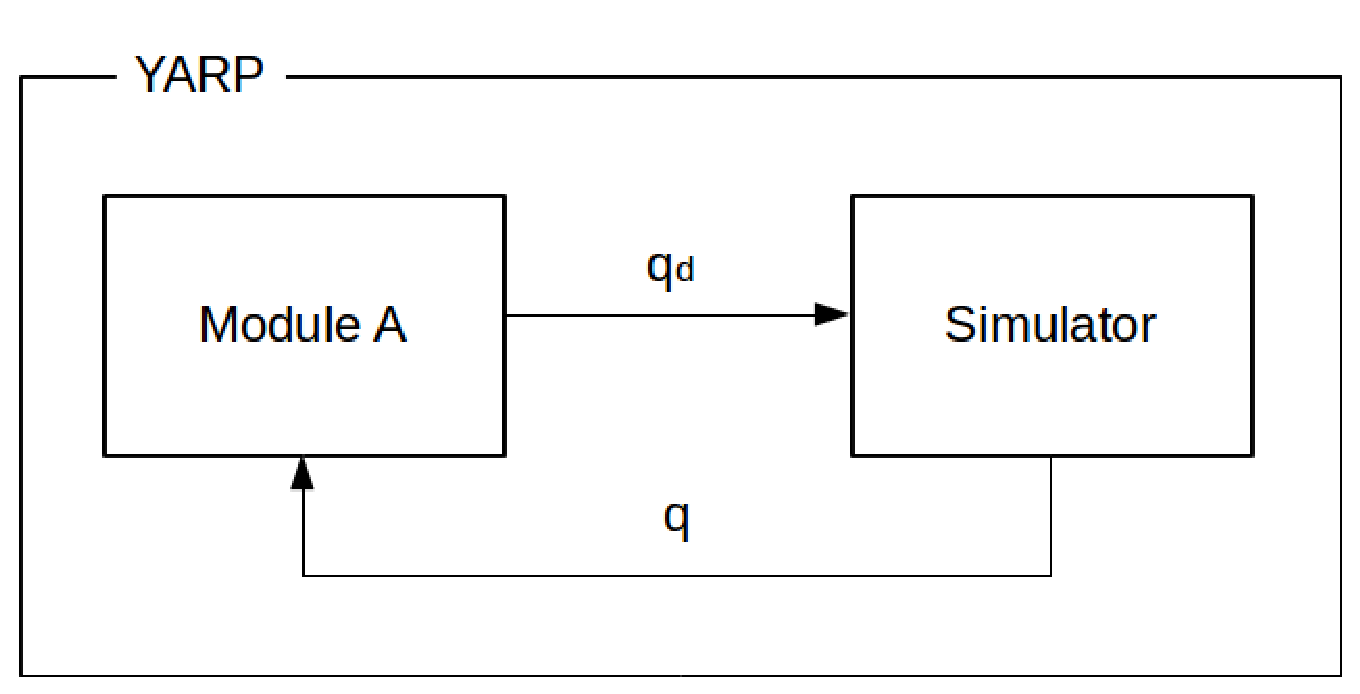
\includegraphics[width=\textwidth]{images/yarp_simulation_a.eps}
                \caption{Module A connected to the simulator}
                \label{yarp_simulation_a}
        \end{subfigure}%
        \\
        \begin{subfigure}[b]{0.45\textwidth}
                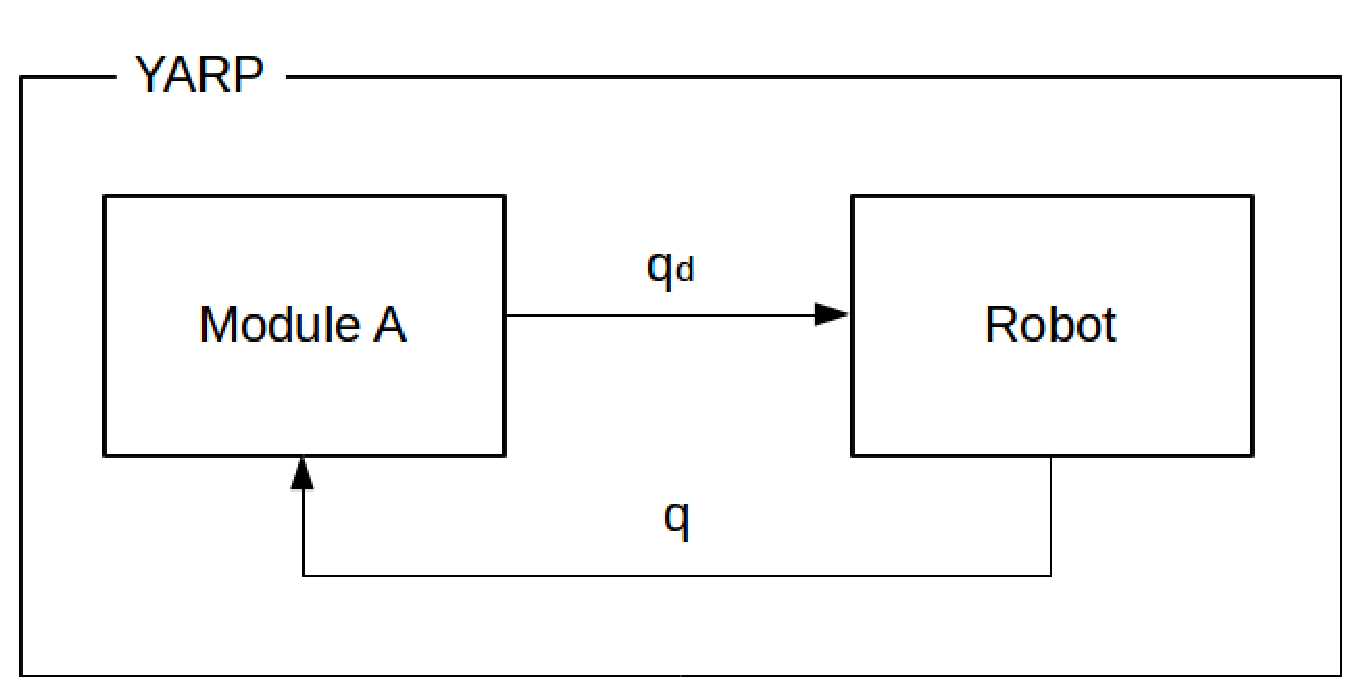
\includegraphics[width=\textwidth]{images/yarp_simulation_b.eps}
                \caption{Module A connected to the robot}
                \label{yarp_simulation_b}
        \end{subfigure}
        \caption{Module A write desired joint position and read actual joint position without knowing if it is interfaced with the simulator or the robot since they expose the same interface.}\label{yarp_simulation}
\end{figure}

A preliminary stage of simulation during development of both research and production code, has many benefits that increase as the cost of production and maintanance of the hardware increases. Moreso, the ability of seamlessly switching between simulator and robot is an important factor that helps reduce development time and is not prone to errors and artifacts introduced during porting, enabling validation by simulation.
Also the simulator provides fundamental advantages, like the ability to simulate faster than real-time.

\subsection{Related Work}\label{related_work_simulators}
The \emph{Open Dynamics Engine} (ODE, \cite{opende}) is one of the most widely used rigid body dynamics engine in robotics simulation. ODE simulates chains of rigid bodies connected and constrained by different types of joints. It has a built-in collision detection system and implements hard contacts using non-penetration constraint whenever two bodies collide. Beside the large number of project that use it, at the moment the development has been paused. \emph{Bullet} (\cite{bulletpe}) is another dynamic engine. It implements different direct/inverse rigid body dynamic algorithms (eg. Featherstone articulated body algorithm, \cite{Featherstone:2007:RBD:1324846}) as well as different solvers (eg. Mixed Linear Complementarity Problem, MLCP) and contact models. Bullet is used for a wide range of projects and its community is active and continues to improve it constantly.

\emph{OpenRAVE} (\cite{diankovthesis}), \emph{Webots}  (\cite{Michel04cyberboticsltd}), \emph{V-REP} (\cite{conf/iros/RohmerSF13}) and OpenHRP  (\cite{journals/ijrr/KanehiroHK04}) all use the aforementioned dynamics engine, or variations thereof, and differ itself in the offer of libraries that aid in modeling, planning, controlling simulated systems.

The most recent MuJoCo (\cite{conf/iros/TodorovET12}) offers a novel approach to simulating dynamic systems with contact, and performed well comparatively to other simulators in a set of benchmarks\cite{erez15}.

In particular, in the last years, we have been witness to the significant investment in resources to provide reliable simulation tools for humanoid robots~\cite{Hsu14} which has been fostered by the Darpa Robotics Challenge (DRC). The results of this investment has allowed teams to compete virtually before qualifying for expensive robot hardware.  
Gazebo~\cite{koenig2004design} is one of the most popular general-purpose robot simulators, funded through DRC efforts.
It is a generic multi-robot simulator, historically developed taking into account simulations in outdoor environments, and especially interesting nowadays for its high level of integration, as it provides realistic simulation of sensory feedback. including noise modeling. Other than ODE and Bullet, it allows to use DART \cite{DART} and the promising SimBody \cite{Sherman2011241}, which is the only supported engine at the moment implementing variable step integration. For these reasons, and for its complex high level architecture, Gazebo has been used to compare algorithms for navigation and grasping in a controlled environment.
To this day, its development is mainly performed by the Open Source Robotics Foundation (OSRF) under an open-source license, and is supported by a very large community.

Gazebo is expandable by means of its plugin structure: thusly our YARP interface to the Gazebo simulator is a collection of plugins, the \emph{gazebo\_yarp\_plugins}, that offer features wich will be described to various degrees of detail in the current section. 


\subsection{Software Architecture}\label{structure}
Gazebo plugins are C++ classes that extend the functionalities of Gazebo, while YARP device drivers are C++ classes used in YARP for abstracting the functionality of robot devices.
Usually, each class of gazebo\_yarp\_plugins embeds a YARP device driver in a Gazebo plugin. 

{\bf Gazebo Plugins}
A plugin is a piece of code compiled as a shared library and inserted into the simulator. A plugin has direct access to all the functionalities of Gazebo from the physics engine to the simulated world. There are 4 types of plugins in Gazebo: \textbf{world}, \textbf{model} and \textbf{sensor} plugins are attached to and control a specific simulated world/model/sensor respectively, while \textbf{system} plugin are specified on the command line and loads during the Gazebo startup.


{\bf YARP \emph{Device Drivers}}
YARP provides special devices that act as network proxies and make interfaces available through a network connection. This allows accessing devices remotely across the network without code change.

A device driver is a class that implements one or more interfaces. There are three separate concerns related to devices in YARP:
\begin{itemize}
\item Implementing specific drivers for particular devices
\item Defining interfaces for device families
\item Implementing network wrappers for interfaces
\end{itemize}
For example the Control Board device driver implements a set of interfaces that are used to control the robot (IPositionControl, ITorqueControl, etc.) and another set of interfaces to read data from the motors (IEncoders, etc).

\subsubsection{Gazebo-YARP Plugins}
The gazebo\_yarp\_plugins is composed of:
\begin{itemize}
    \item Gazebo plugins that instantiate YARP device drivers,
    \item YARP device drivers that wrap Gazebo functionalities inside the YARP device interfaces.
\end{itemize}
The plugins/devices implemented are the \emph{Control Board}, \emph{6-axis Force Torque sensor}, \emph{Inertial Measurement Unit} (IMU) and a \emph{Clock} plugin used for synchronization. The plugins stream data which is generated by the Gazebo simulator, and thus support all the features of the simulator, such as modelling Gaussian noise on the IMU readings.
While the first three plugins are directly related to the simulated objects and sensors, the last one is a system plugin that synchronizes the YARP modules with the simulation time.

\begin{figure}
        \centering
        \begin{subfigure}[b]{0.475\textwidth}
                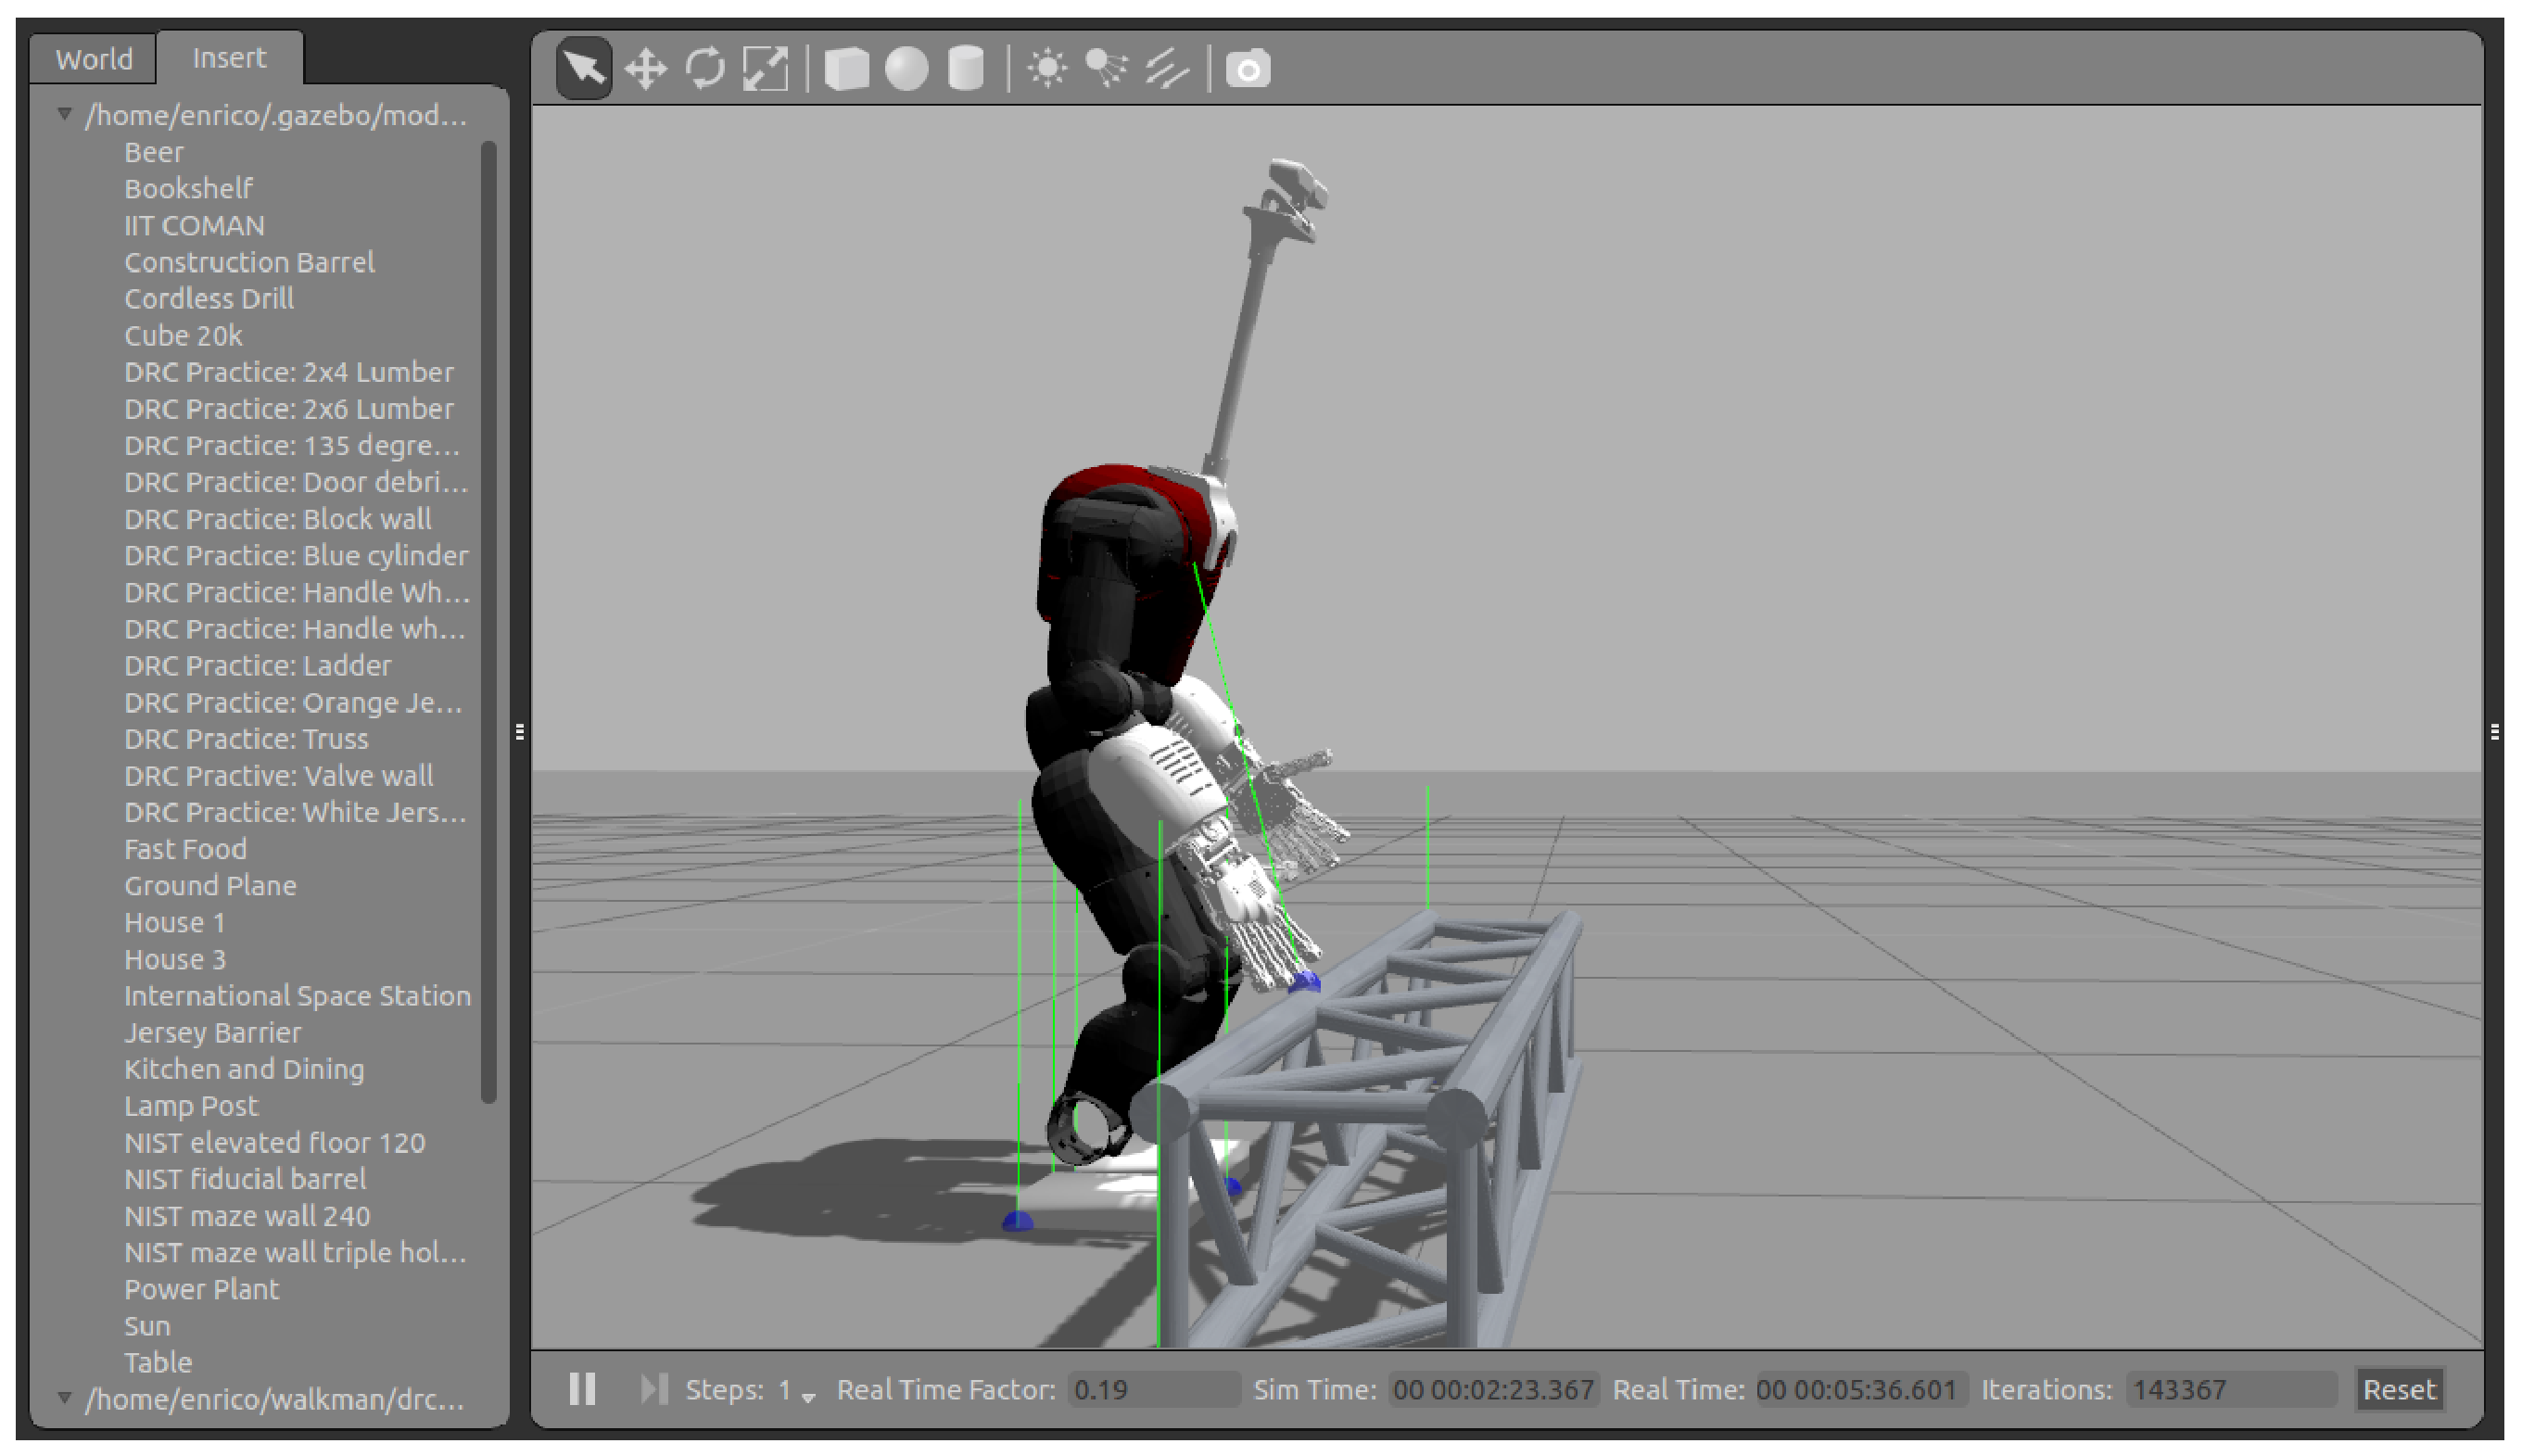
\includegraphics[width=\textwidth]{images/coman_ft_a.eps}
                \caption{Gazebo interface with COMAN}
                \label{yarp_simulation_coman_a}
        \end{subfigure}%
        \\
        \begin{subfigure}[b]{0.475\textwidth}
                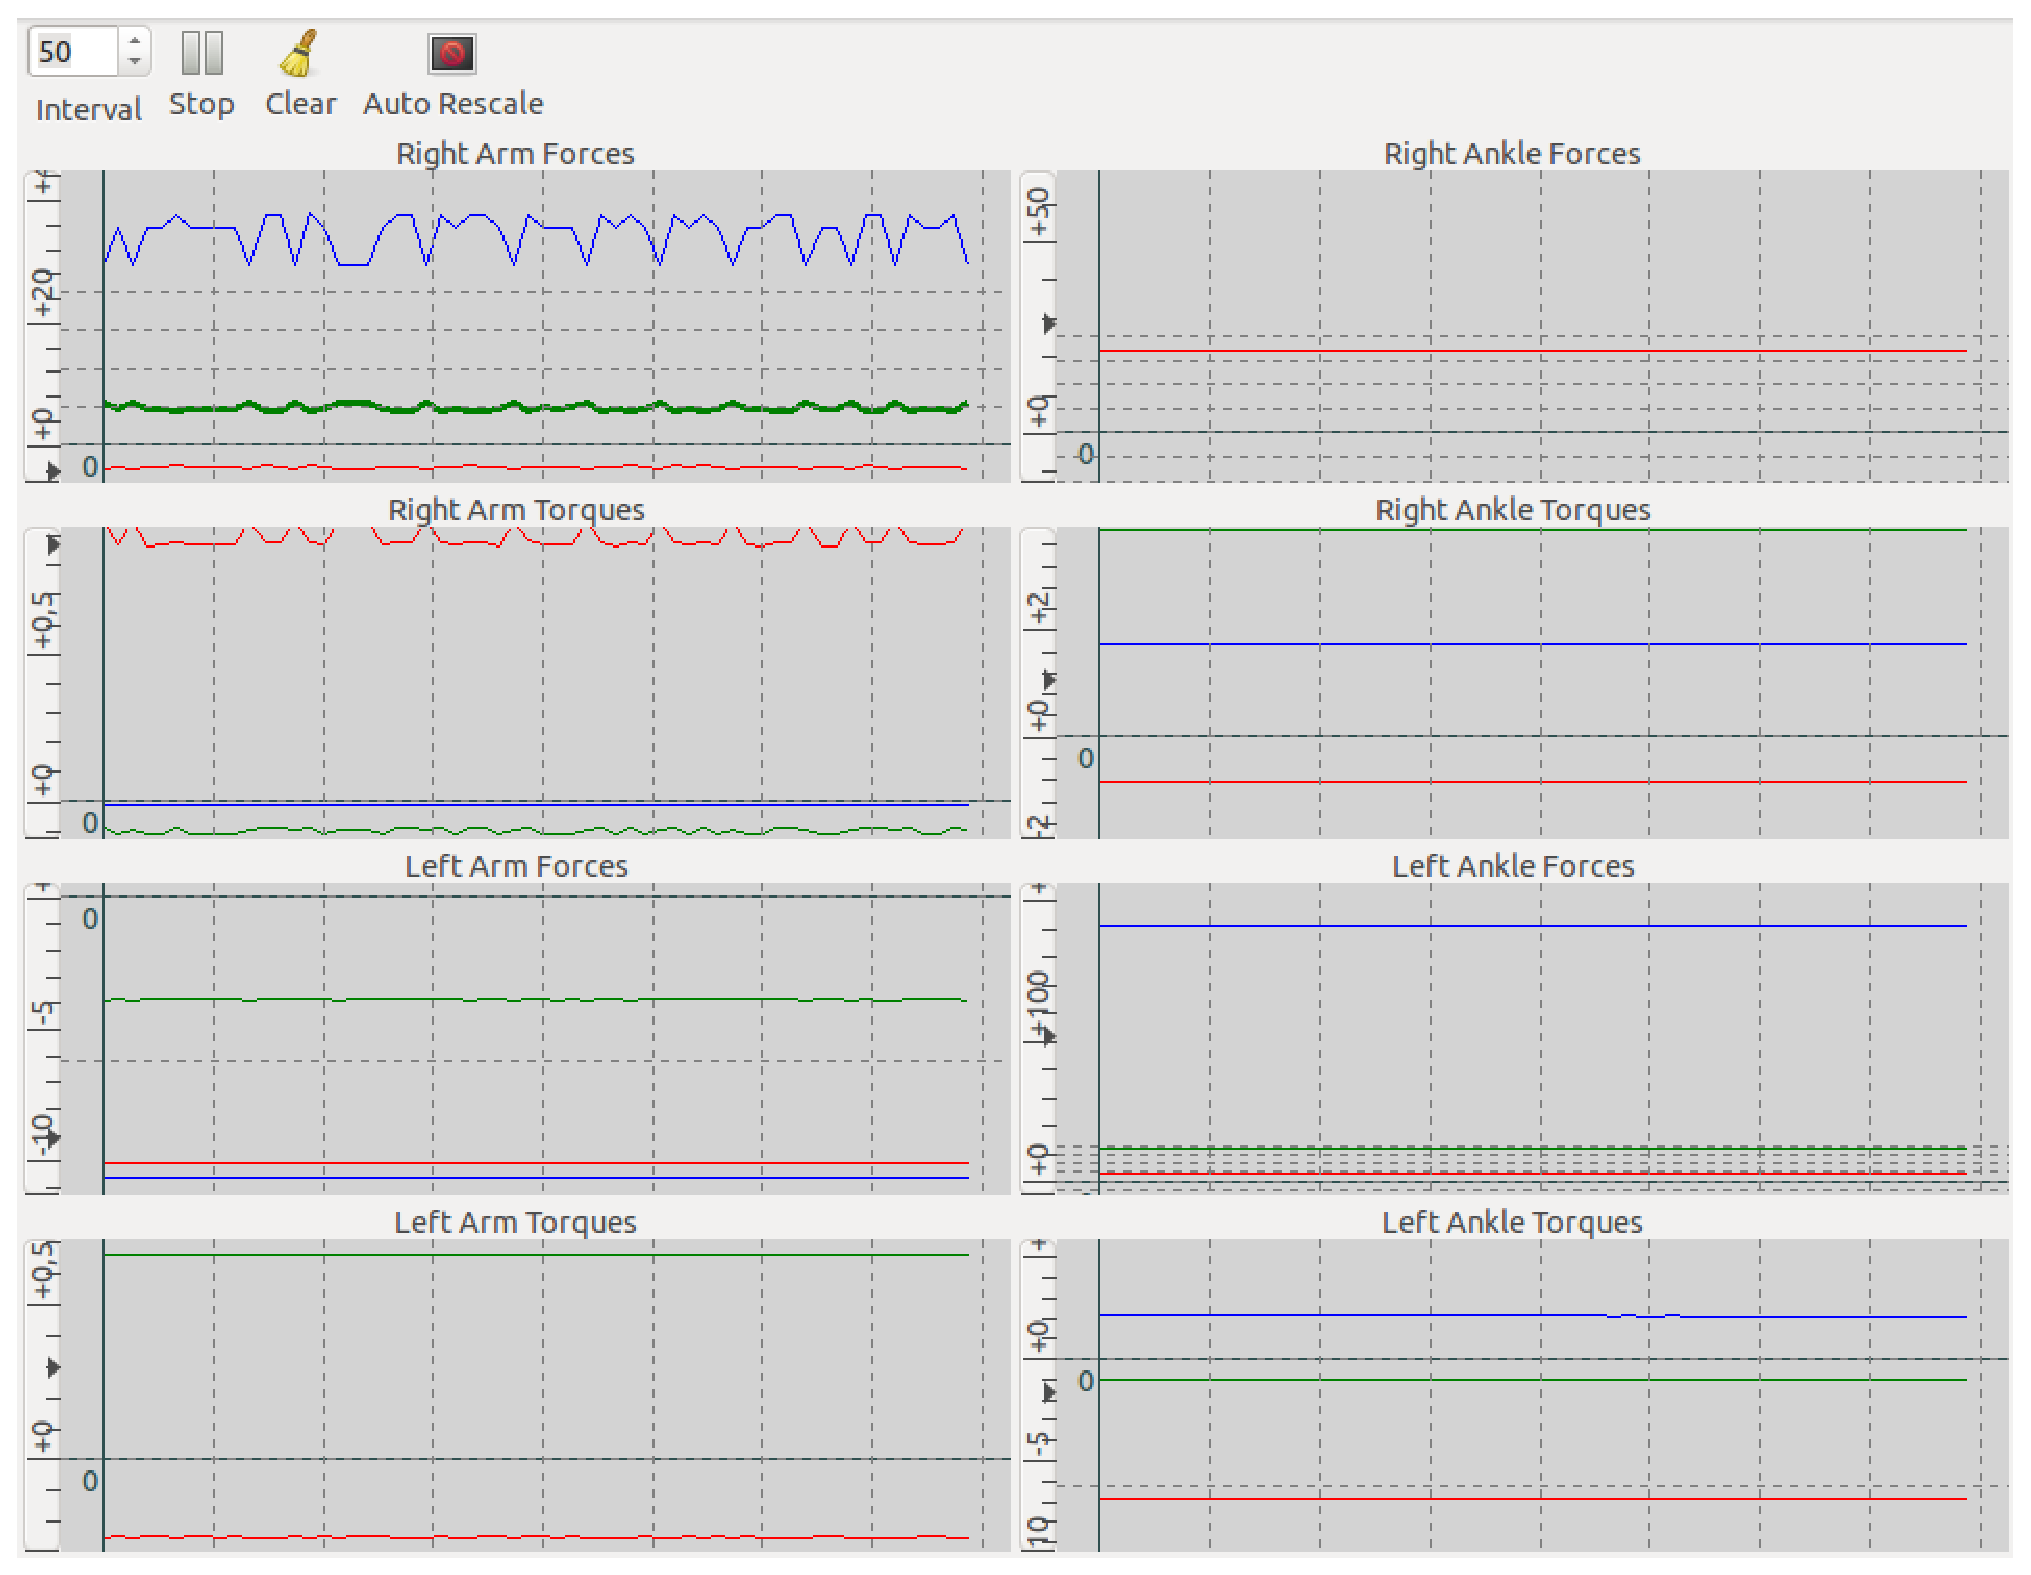
\includegraphics[width=\textwidth]{images/coman_ft_b.eps}
                \caption{A yarpscope showing on-line the forces and the torques at each Force/Torque sensor}
                \label{yarp_simulation_coman_b}
        \end{subfigure}
        \\
        \begin{subfigure}[b]{0.475\textwidth}
                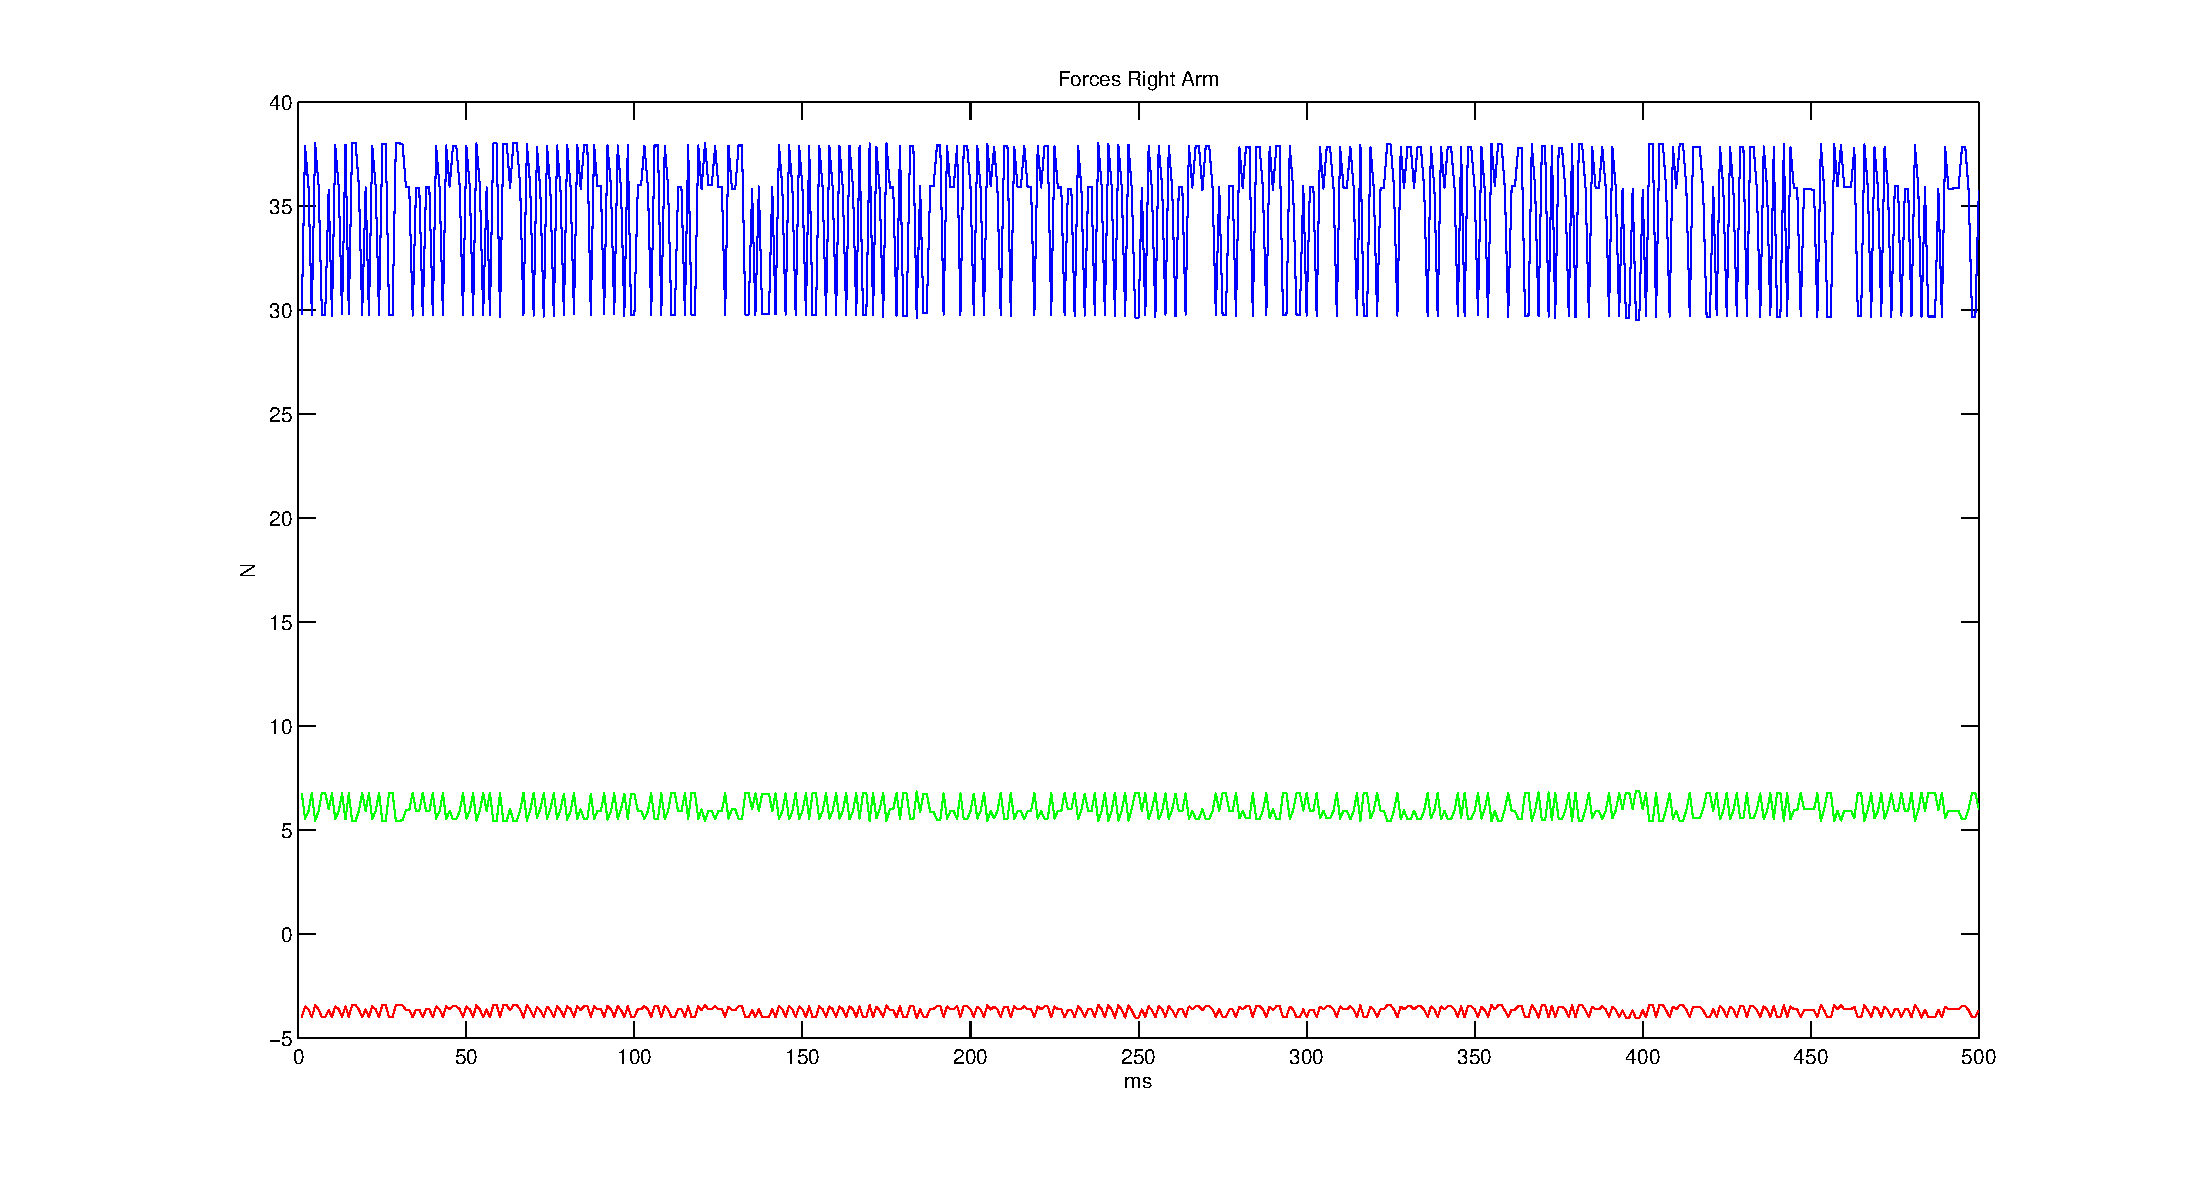
\includegraphics[width=\textwidth]{images/coman_ft_c.eps}
                \caption{Plot of forces measured at the simulated Force/Torque sensor placed on the right arm. Forces along x,y and z are respectively in red, green and blue}
                \label{yarp_simulation_coman_c}
        \end{subfigure}
        \\
        \begin{subfigure}[b]{0.475\textwidth}
                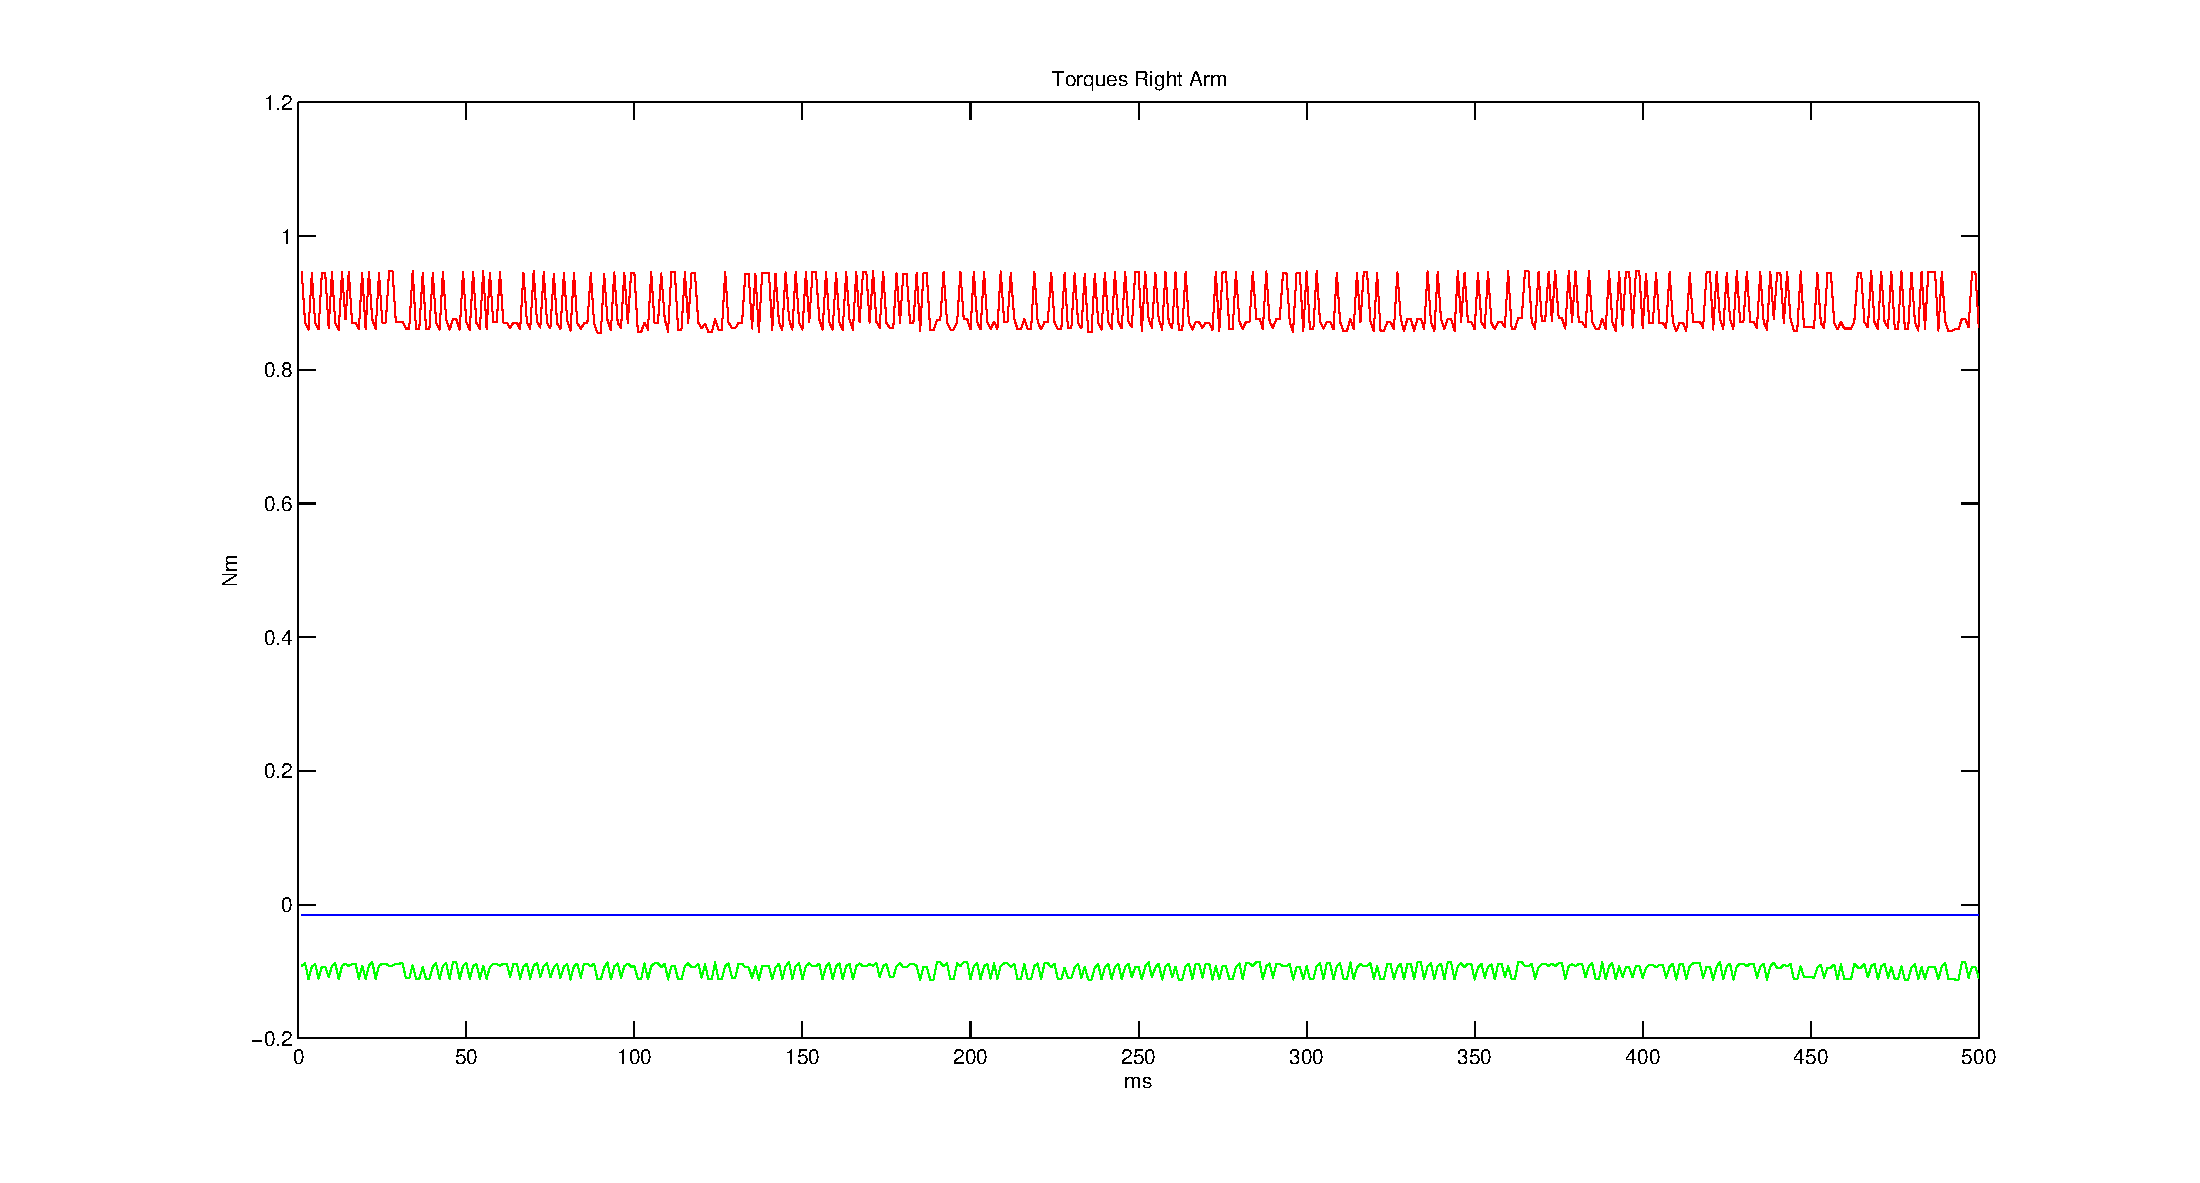
\includegraphics[width=\textwidth]{images/coman_ft_d.eps}
                \caption{Plot of torques measured at the simulated Force/Torque sensor placed on the right arm. Torques along x,y and z are respectively in red, green and blue}
                \label{yarp_simulation_coman_d}
        \end{subfigure}
        \caption{A Gazebo simulation running COMAN interacting with debris}\label{force_torque}
\end{figure}

\subsubsection{Control Board}
The Control Board plugin allows to control the robot using YARP Interfaces, it is implemented as a Gazebo Model plugin. Every control board allows the user to control one or more joints (a kinematic chain such as the arm or leg, etc.) as specified in a configuration file. For each controlled joint the control board opens different interfaces, permitting the use of different type of controllers for each joint. Such interfaces include position control, torque control, encoders reading, torque measurement and joint impedance control. Usually the number of instantiated control boards is equal to the number of kinematic chains.
This duality between control boards and kinematic chains can be abandoned for the sake of performance on the real hardware, since every control board is usually implemented by a thread that streams data in a specified port. In that case, typical whole-body control then has to collate the network data coming from each control board and infer the global state of the robot. Each control board, during every cycle of simulation, reads position, velocity and torque values from the simulated joints and sends desired joints position or torques to the simulator. The values read from the simulator are broadcasted through YARP interfaces in the YARP network, in a similar way the desired joint values come from YARP interfaces (Figure \ref{control_board}). The following YARP interfaces are used to control the robot.
\begin{itemize}
\item \textbf{IPositionControl}: a position control with a linear trajectory generator considering a max joint speed
\item \textbf{IPositionDirect}: a position control using Gazebo position PIDs
\item \textbf{ITorqueControl}: a perfect torque follower
\item \textbf{IImpedanceControl}: a joint impedance control with the following law
\begin{equation}
    \tau_d = -P_d(q-q_d) - D_d\dot{q} + \tau_{offset}
\end{equation}
where $q_d$ is the desired equilibrium position, $P_d$ is the desired joint stiffness and $D_d$ is the desired joint damping. $\tau_{offset}$ is an extra term that can be used for gravity compensation or inverse dynamics control.
\end{itemize}
Furthermore, the Control Board implements the \textbf{IControlMode} interface that allows to change the type of controller online. All these interfaces are also available on the robot and they have the same behaviour.

\begin{figure}[h!]
  \centering
    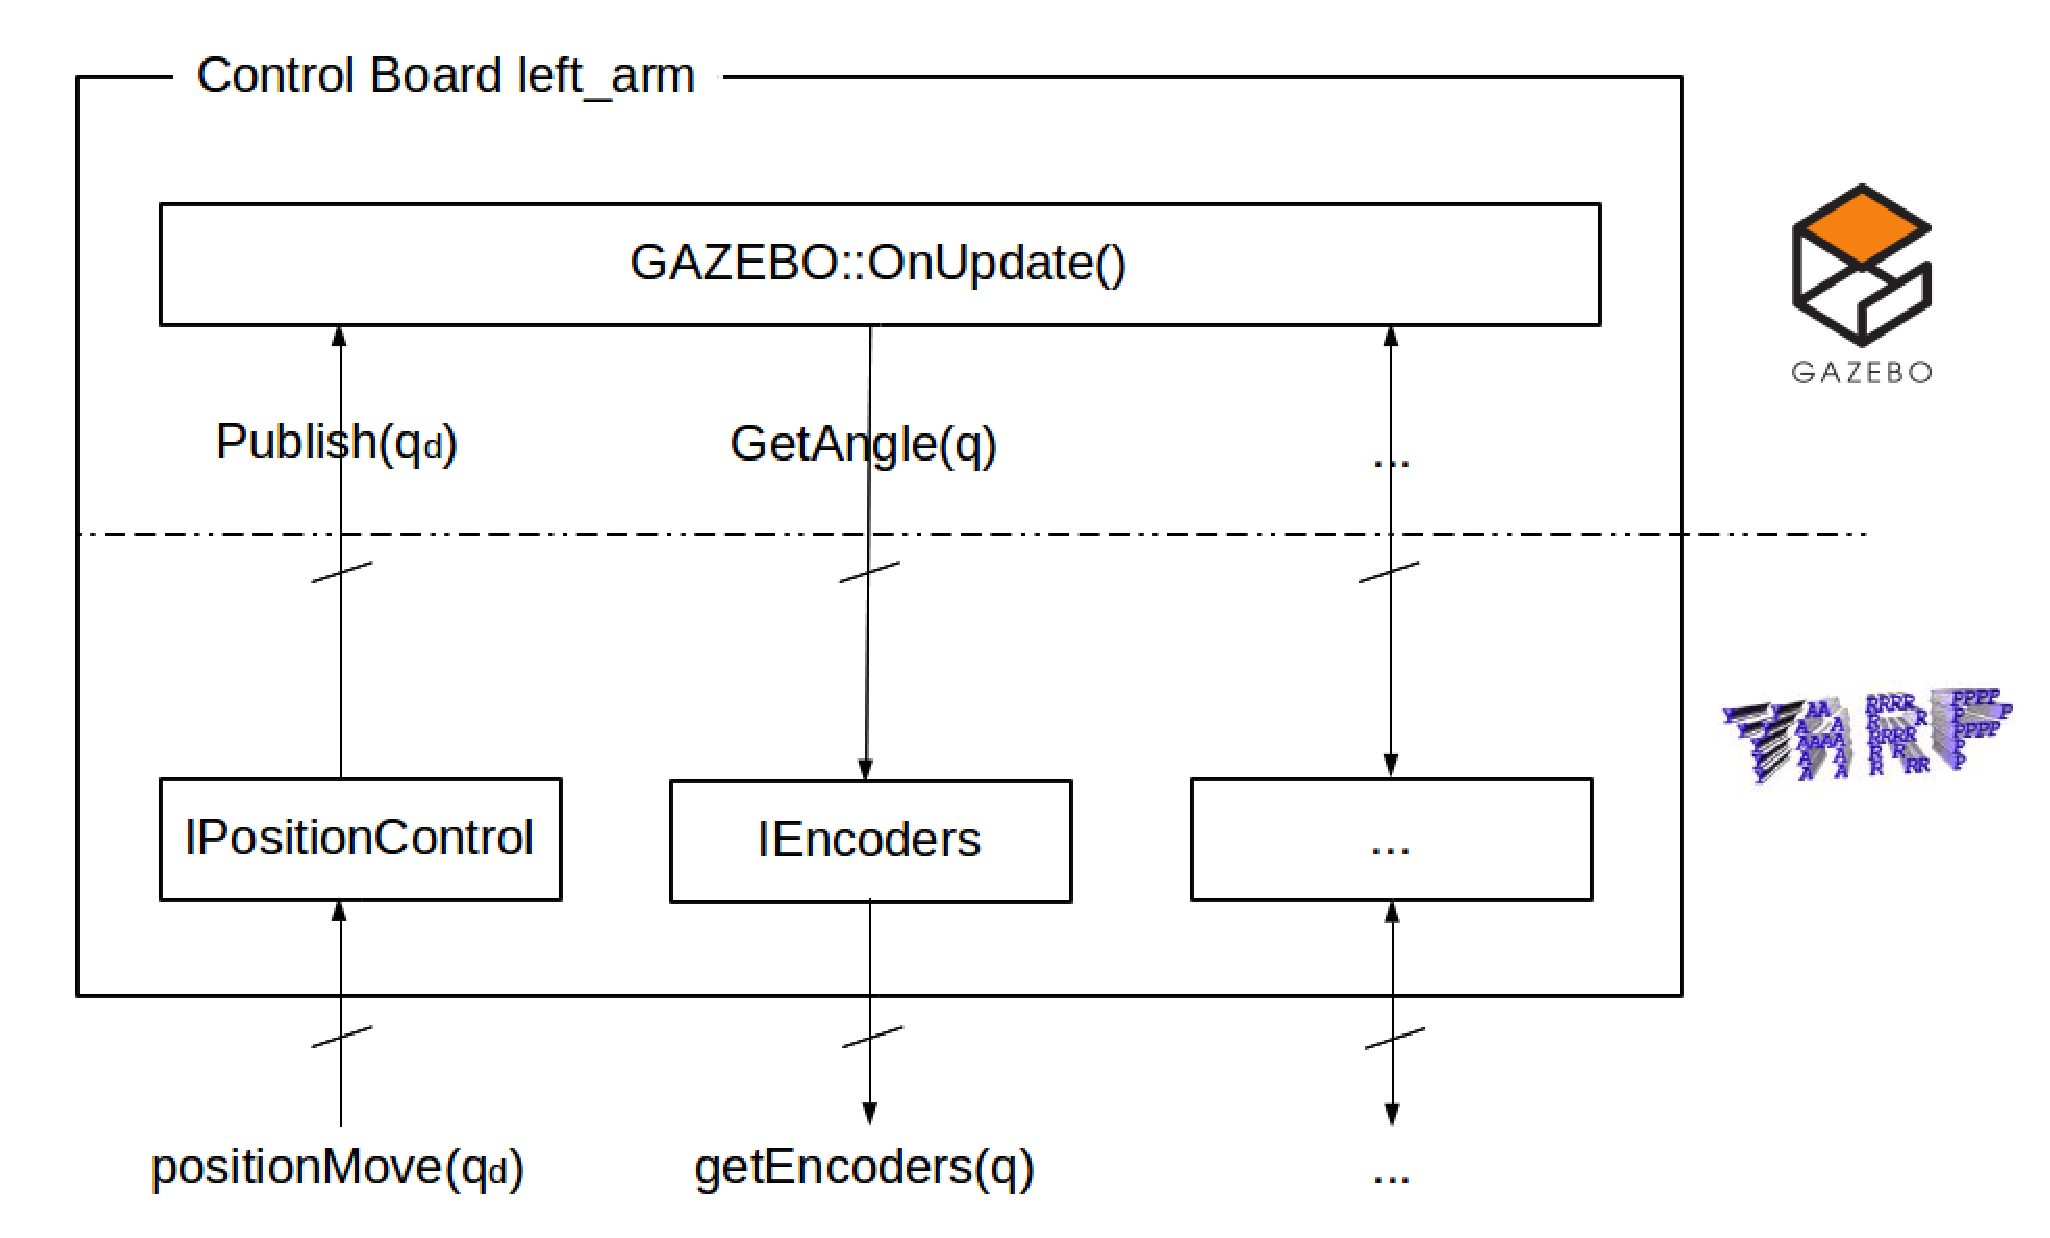
\includegraphics[width=0.5\textwidth]{images/control_board.eps}
    \caption{Control Board plugin for the left\_arm kinematic chain. yarp::IPositionControl interface has a method positionMove() that can be used to set joint values inside a YARP module. The plugin implements such interface by calling the Publish() method inside the Gazebo API to move the simulated joints at each OnUpdate().}\label{control_board}
\end{figure}

\subsubsection{6-axis Force/Torque sensor}
A Force/Torque sensor measures a wrench in the robot structure (Figure \ref{force_torque}). The sensor streams the data that are provided by Gazebo from a joint information. In fact, simulators like ODE use a maximal coordinate system, meaning that every body is simulated as an unconstraied ribid body (6DOFs), where constraints are enforced through the LCP formulation. This makes so that also joints are constraints, and since during simulation tipically the solver allows for constraint violation to a certain degree, which is proportional to the forces acting on the system and the equivalent stiffness of the constraint, such violation can be used to infer the forces and torques acting on the joint. \todo{add more details about the stiffness of joints} On the YARP side, the reading of a generic sensor is implemented as a \textbf{IAnalogSensor} interface (Figure \ref{ianalog_force_torque}). The broadcasted data is a vector of six numbers representing the forces and the torques applied on that reference frame.

\begin{figure}[h!]
  \centering
    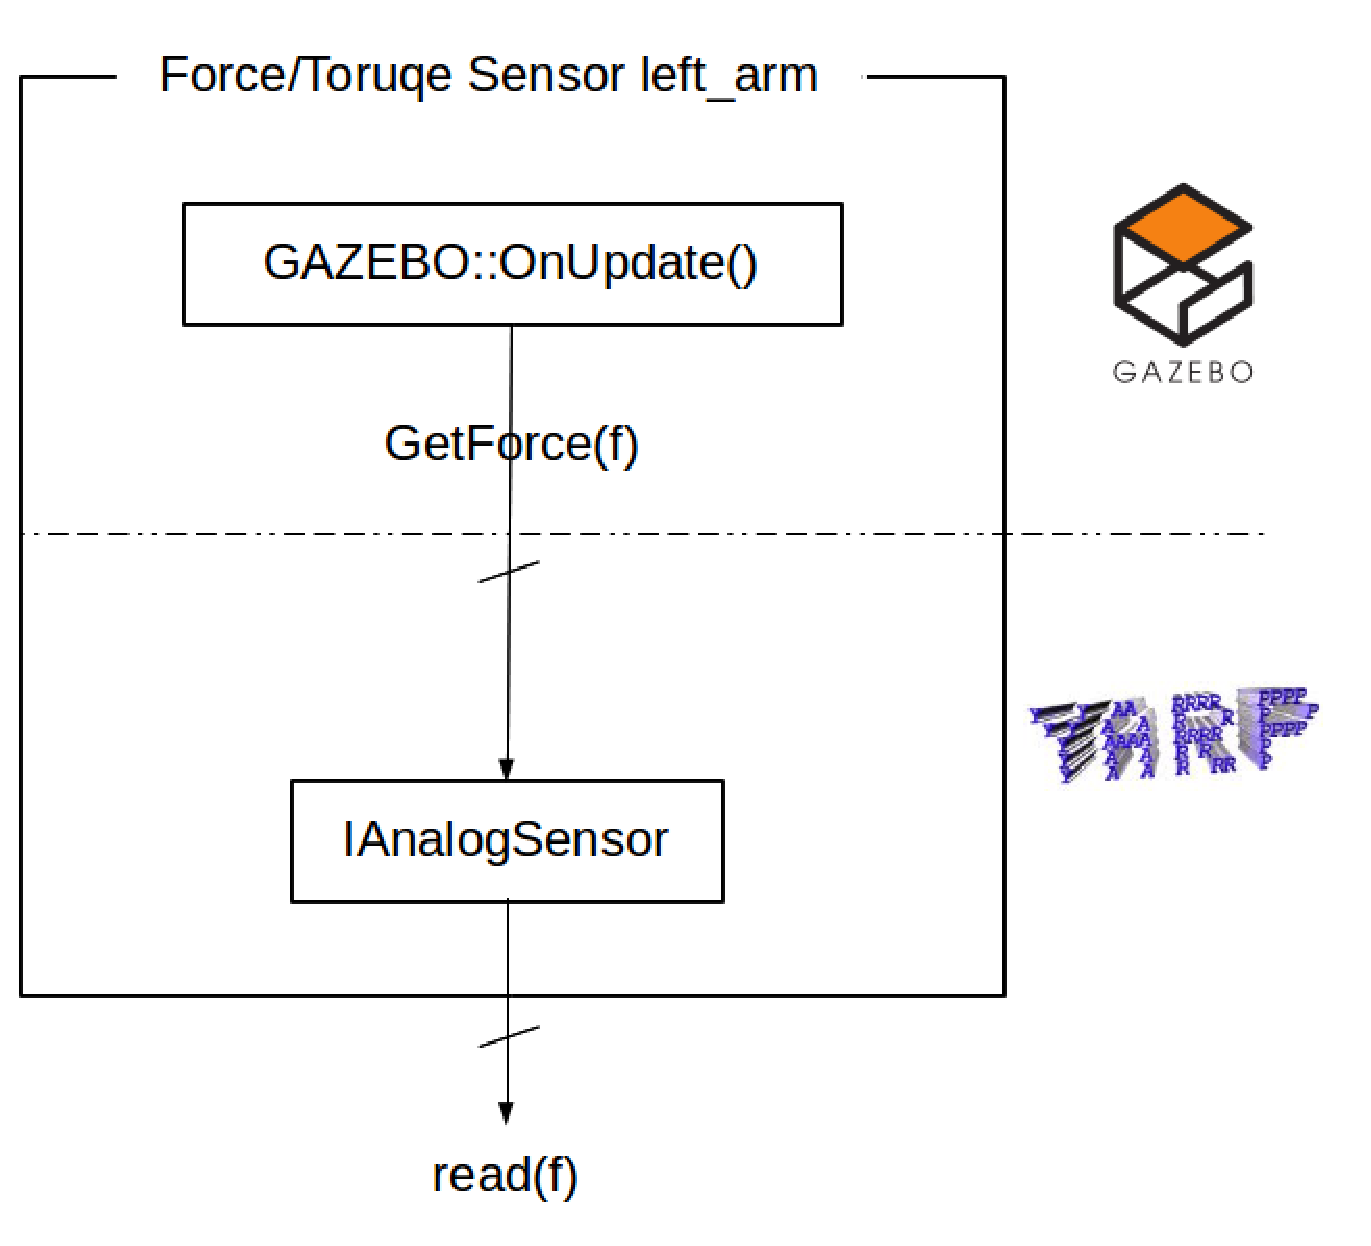
\includegraphics[width=0.475\textwidth]{images/ianalog_force_torque.eps}
    \caption{The Force/Torque sensor in the left arm is implemented as a YARP IAnalogSensor interface. At every step the internal state of the plugin is updated with the last readings of forces and torques from the simulation.}\label{ianalog_force_torque}
\end{figure}

\subsection{Real-Time Simulation of Robotic Systems: Clock}
\begin{figure}
  \centering
    \hspace*{-0.25in}
    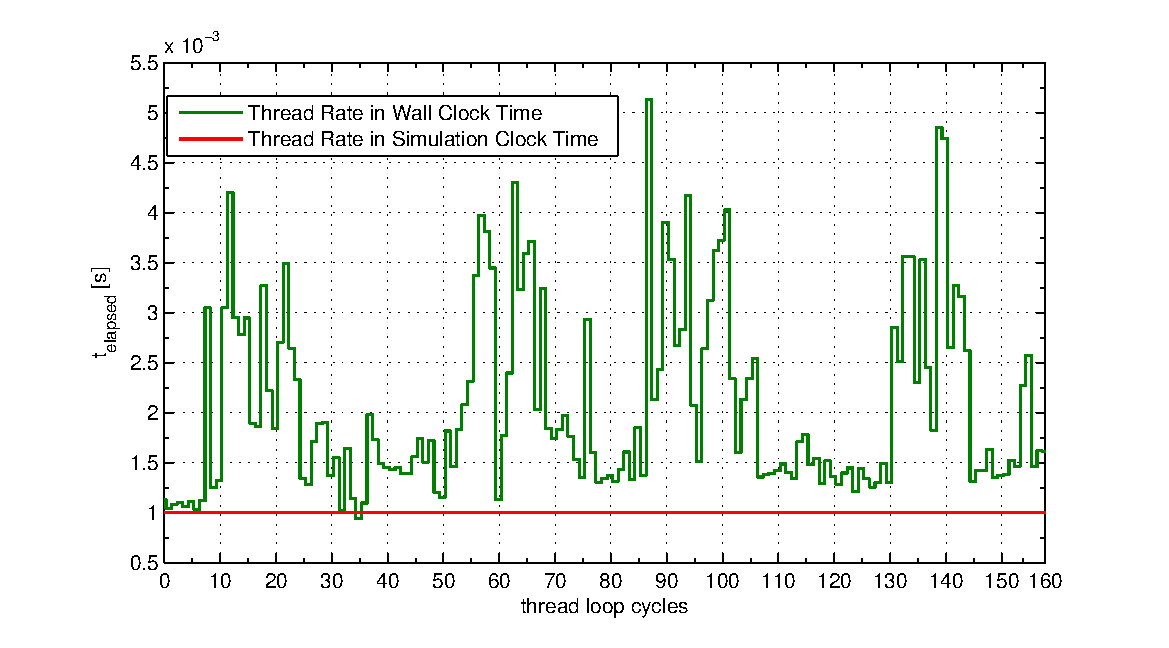
\includegraphics[width=0.51\textwidth]{images/yarp_clock.eps}
    \caption{Time elapsed between each execution of the control loop, measured in simulation clock time and in wall clock time. Desired thread rate is $1$kHz and simulation time step is $1$ms}\label{yarp_clock_real_vs_simulated}
\end{figure}
A fundamental aspect of simulation is the synchronization between the simulation code and the high level task code. Often, ad-hoc solutions emply a simulator-in-the-loop approach were after a certain number of simulation steps, and possibly each step, a control step is executed. In this case, we have true bidirectional synchronization between the simulation and the task code, that is, locked-step simulation. Since our code needs to be indipendent and agnostic of the simulator, it needs to be a networked application, and a synchronization mechanism needs to be put in place. In particular, the low level control algorithms specified in \ref{control_board} is automatically synchronized with the simulation, and mimics the real-time characteristics of the low-level decentralized control running on the joint's boards of a robot. In order to simulate also real-time execution of the high-level code, synchronization between YARP modules and the simulated robot is needed.
A YARP module is a process in which one or more threads are started. When such modules are used in the real robot, the thread rate is timed by the machine (system) clock, also called the \emph{wall clock}. In the same way, the client code's loop needs to be synchronized to the simulated clock when controlling a simulated robot.
The \emph{real-time factor} (\emph{RTF}) of the simulation is given by 
\begin{equation}
    RTF = update\_frequency \times step\_time
\end{equation}
and is kept to one when the desired update frequency is the inverse of the time increased at each step in the simulation.
%because if the real time factor of the simulation is above 1.0 the control could run in general faster than the simulation and this is not realistic. 
For instance if the simulation runs with a real time factor of 0.1, 10 seconds are needed to simulate $1$ second of the physical system evolution. Within this situation, the controller process should also be slowed down 10 times to be coherent with the simulation. To solve this issue a \emph{clock} plugin has been designed that synchronizes the high level control modules with the simulated time when controlling a simulated robot. The idea is similar to the ROS clock plugin for the Gazebo simulator, in that it is not a lock-step synchronization, meaning that in order to run the simulation faster than real-time we need the control code to be fast enough, since the control code will be synchronized with the simulation clock but the simulation will not wait for the control code to complete execution before starting the next simulation step.

The \emph{clock} plugin is implemented as a System plugin and publishes on a YARP port the time information from the simulator. For every simulation step, the simulation time is incremented and the timestamp is sent via socket. The data sent via this port acts as signal for a $1$Khz simulated scheduler that wakes up the control threads that need to be woken up.

In general, all the YARP functions that provide access to the computer internal clock and support thread scheduling can be synchronized with an external clockof choice, be either coming from the simulator or other means (this is enabled with the \emph{YARP\_CLOCK} environment variable). Classes supporting periodic threads (\emph{RFModule} and \emph{RateThread}) are therefore automatically synchronized with the clock provided by the simulator. The \emph{yarp::os::Time} functionalities are also transparently working using the wall-clock or the simulation clock depending on the environment variable. Thread sleeps are performed using the wall or simulated time depending on the circumstance.

More in detail, when synchronized with the simulation clock the \emph{yarp::os::Time} delay does not explicitly sleep on a wall clock, rather a scheduler is synchronized with the simulation clock by performing blocking reads on the \emph{YARP\_CLOCK} port. This scheduler wakes up the threads that required a delay just once, when they have slept for the desired duration. Compared to the ROS::Time implementation which uses small sleeps on wall clock to check synchronization with the simulated clock, this allows to run simulations both slower and faster than real time and still have synchronization between threads and controls. In any case, when accessing the simulated clock Experiments showed the approach to be successful in synchronizing $1$kHz control loops against simulations running $1$kHz, thus having a $1$ms clock granularity.

A similar solution for synchronization has been consequently used also in \cite{wbi14}.

\subsection{Notes on Simulation of compliant, highly redundant robots}
The problem of simulating compliant humanoid robots in particular, and highly redundant robots in general, is the computation burden due to the large amount of joints (and thus, rigit bodies) that need to be simulated.
Work is ongoing to properly simulate these systems on Gazebo, by using the Spong model and effectively doubling the number of simulated joints.\todo{input Spong Equation} While this approach allows to accurately simulate robot compliance but poses performance problems.
A practical approach that has been used for the simulation of the robots developed at the Istituto Italiano di Tecnologia that are equipped with SEA joints, in particular when used in position control schemes, has been to tune the system PIDs to the actual joint compliance in the robot. Assuming a perfect controller on the physical robot, and taking into account that the simulated PID has a torque feedback, then the P gain is dimensionally a stiffness, and the D gain is a damping.
Technically, simulating compliant robots is easier than simulating stiff systems, were implicit integration schemes are needed for stability. \todo{cite ref}
The current Gazebo simulator uses a semi-implicit integration scheme, nonetheless simualaing very rigid robots (through very rigid PIDs) requires small integration steps, which compromise simulation speed. In our experiments, simulation is always run with a $1$ms timestep.

\subsection{Conclusions}
In this section we have presented a set of Gazebo plugins, named \emph{gazebo\_yarp\_plugins}, that allow to connect the robotics framework YARP to multi-purpose simulator Gazebo. Gazebo was chosen since it is easy to use, it has the possibility to switch between different rigid multi-body dynamics engines, it is Open-Source and has an active community. Our plugins are based on YARP device drivers in order to have the same interfaces in the real and simulated robot. This allows to write modules that will work both in the simulator and in the real robot without the need to modifiy the code. This is a very important paradigm in robotics since it minimizes the chance of introducing errors due to porting of the code, and allows for automatic validation by means of simulation. Furthermore the simulator becomes a tool that helps the developer in testing and validating before using the real platform.
Such plugins consist in: a Control Board plugin to control the robot, a Force Torque sensor plugin and an IMU plugin. A special plugin dedicated to synchronization between modules and simulator was also implemented. The plugins were tested to simulate several humanoid bipedal robots, including the COMAN, iCub, and WALKMAN from the Istituto Italiano di Tecnologia.


%%%%%%%%%%%%%%%%%%%%%%%%%%%%%%%%%%%%%%%%%%%%%%%%%%%%%%%%%%%%%%%%%%%%%%%%%%%%%%%%
\section{Simulating Grasps}

Despite increasing popularity of compliant and underactuated hands, there exist few analytical and simulation tools for modeling such hardware.  High-fidelity predictive tools are important in mechanism design as well as grasp planning and optimization to exploit the favorable features of compliant hands.

The following section will report studies \cite{Rocchi2016-jq} on a variety of simulation techniques to predict the success of a compliant gripper on irregular objects.  In particular, performances of a new simulator will be presented, that integrates compliance simulation with a recent Boundary Layer Expanded Mesh (BLEM) technique for enhancing stability of contact normal and penetration depth estimation.
The novel simulator is compared against existing ones using a set of stability and fidelity indices: \emph{contact force smoothness} and \emph{contact position and normal stability}.
Scores along these indices are correlated with the simulator's accuracy of predicting the success/failure of a given grasp pose and preshape.  
A testing set of 13 grasps of varying success rate on physical hands were manually generated for the  \emph{RightHand Robotics} \emph{Reflex Hand} and \emph{Pisa-IIT} \emph{Soft Hand} on $4$ objects with a known 3D model and mass distribution. 
Each grasp is simulated using multiple techniques, and experiments find that the novel simulator leads to improvements both in the stability indices, predictability of grasp success, and reduction of simulation artifacts.

The critical point of the evaluation lies on defining appropriate metrics, which can be considered universal in assessing the capabilities of a grap simulator to predit the behavior of compliant grippers grasping rigid objects. The physical and simulated experiments also have been designed to both highlight the importance of contact stability and accuracy during grasping (e.g. picking grasp poses where object ridges and geometric qualities of the object influennced the grasp outcome), and the importance of correctly simulating compliance (e.g. scenarios where the objec lies on the table and the hand fingers need to slide on the surface to perform a cage grasp).
%is susceptible to contact stability, that the \emph{BLEM + hierarchical clustering} provides the best indices over the set of techniques presented, and illustrate some examples where a physical grasp grading can give unique insights over the stability of grasps empowered by environmental constraints, grasps of kinematic chains, and grasps of objects where the mass distribution is known.

\subsection{Stable Simulation of Underactuated and Compliant Hands}
%%%%%%%%%%%%%%%%%%%%%%%%%%%%%%%%%%%%%%%%%%%%%%%%%%%%%%%%%%%%%%%%%%%%%%%%%%%%%%%%
\begin{figure}[!hbt]
\begin{center}
        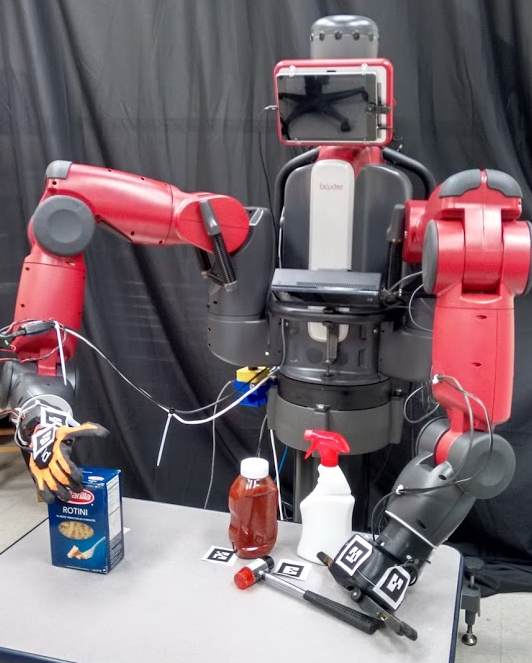
\includegraphics[width=0.75\columnwidth]     {images/ssoch/baxter_HDR}
        \caption{the Baxter robot equipped with a Reflex Hand and a Soft Hand with the gasp set used for the experiments}
        \label{fig:baxter}
        \end{center}
\end{figure}
%[KH: Irrelevant]
%In recent years, the variety and complexity of robotic hardware has been influenced by the steady rise of rapid prototyping tools, and started to move from lab-spaces to real environments while requiring designs to be cheaper and more robust.
An increasing number of robot hand designers have been moving towards devices that make use of compliance and underactuation. The iHY~\cite{Odhner14}, Reflex Hand~\cite{ReflexHand}, Pisa/IIT SoftHand~\cite{Catalano14}, Robotiq 3 fingers gripper~\cite{Robotiq3Finger}, RBO~\cite{Deimel13} and RBO2~\cite{Deimel14} and Yale Hands~\cite{Ma13} are recent examples of underactuated compliant hands. The main benefits of such designs include hardware robustness and the capability of adapting the hand shape to a wide range of grasped objects. Underactuated hands provide many degrees of freedom of movement (DoFs) while being actuated by just a few degrees of actuation (DoAs), and clever passive mechanisms are designed to coordinate the actuation of multiple DoFs, which simplifies the otherwise complex hand control problem. %[KH: "taming" is too dramatic] taming the complexity of the hand control problem by means of intelligent hardware design.
Although compliant hands are built to be more robust to sensing uncertainties than rigid ones, they typically increase actuation uncertainties. As a result, successful grasping still requires deliberation, particularly for objects of irregular shape or mass distribution. It is also challenging to grasp objects in clutter because fingers may be disturbed by inadvertent contact with the environment or other objects. Hence, model-based predictions of motions and forces can offer powerful insights for hardware design as well as grasp optimization and planning.

Unfortunately, classical models for grasp analysis are poor at predicting the behavior of compliant hands. Classic kinetostatic analysis and kinematic simulation under the quasi-static assumption are inappropriate for studying the deformation of the hand under varying contact forces.  Several researchers have turned to physics-based simulation analysis~\cite{Kappler15, JunggonKim13}, which improves grasp predictability by evaluating hundreds or thousands of trials, in which the simulator explores the range of nondeterministic effects, e.g., external perturbations, pose uncertainty, geometric uncertainty, and joint friction. Reliable simulation is essential for such studies. However, compliant hands pose a challenge for dynamic simulation tools, which often have trouble remaining stable in the presence of multiple frictional (and sometimes sliding or rolling) contacts and stiff internal mechanisms, like springs and tendons. When the object is not considered to be fixed to the environment, object-hand interactions need to be simulated taking dynamics into account, and a faithful representation of contact has to be available in order to detect the making/breaking of contacts, inadvertent contact, and sticking/slipping conditions. 

This paper presents a new physics simulator for compliant hands interacting with rigid objects. It integrates models of compliant elements with recent contributions in robust mesh-mesh contact generation methods.  Compliant elements are modeled as spring-dampers while stiffer elements like tendons are handled using constraints and Baumgarte stabilization\todo{cite or add example}.  To handle mesh-mesh contact, the recent \emph{Boundary Layer Expansion Mesh} \emph{BLEM} method is used, that avoids many simulation artifacts by generating continuously differentiable contact points \cite{Hauser13BLEM}. To handle large number of contacts, contact clustering schemes is employed. Various variations of BLEM are explored against existing contact detection schemes in the popular {Open Dynamics Engine}~\cite{opende} and Bullet~\cite{bulletpe} physics engines. This comparison is particularly meaningful as those same contact detection schemes are used in vast the majority of the robot simulators software introduced in \ref{related_work_simulators} with the exception of MuJoCo and SimBody. Two contact filtering schemes ---  \emph{k-means clustering} and \emph{hierarchical clustering} --- are then compared against the \emph{contact sorting} method implemented in the Gazebo simulator.

Finally, a set of indices is established for characterizing the stability of grasping simulations at the level of contact point and force prediction.  A  series of experiments is performed, comparing grasps performed on the physical hardware against results from a variety of simulation tools. Experiments demonstrate that grasp predictability is found to be correlated to the contact stability indices.  Furthermore, the new simulator is demonstrated to achieve improved fidelity regarding the predictability of grasp success/failure compared to existing off-the-shelf simulators.  
%Dynamic simulation tools face the problem of stability, in  particular contact stability in mesh-to-mesh contact scenarios, and when dealing with systems comprised of elements that span different orders of magnitudes in compliance and inertial parameters.

%%A set of successful and unsuccessful grasps is first hand-picked and performed on the compliant underactuated %The hand pregrasp pose and preshape, in case of the \emph{Reflex Hand}, is stored, and then each grasp is simulated multiple times with pose disturbance from a random distribution.

\subsection{Related Work}\label{related_work_grasp}
{\bf Robot Simulators.}
A few robot simulators and toolkits are specialized in grasping, such as GraspIt!~\cite{Miller04}, OpenRave~\cite{Diankov08OpenRAVE} and OpenGRASP~\cite{Leon10OpenGRASP}, which have built-in functionality for grasp analysis. However, replicability of these prior methods assume complete, precise actuation of the hand.

In~\cite{Bonilla14} a dynamic simulation of the Pisa/IIT Softhand is implemented in the multi-body dynamics simulator MSC Adams~\cite{MSCAdams}. A method to generate pre-grasp palm configurations w.r.t. the object pose is provided. The simulator demonstrated moderate fidelity to an experimental scenario, but the authors acknowledge difficulties with hand-object penetrations and estimation of contact normals.

 A recent contribution in the Klamp't simulator is the notion of boundary-layer expanded meshes (BLEM) which were demonstrated to enable robust mesh-to-mesh contacts, even in the presence of non-watertight meshes~\cite{Hauser13BLEM}. In this work we extend Klamp't to handle compliant mechanisms, and also we adapted the BLEM technique into Gazebo as a plugin.

%[KH: this paragraph is irrelevant]
%While simulation is considered by some an ineffective tool for high fidelity prediction of physical systems due to model uncertainty, still it can provide many insights and can be used with success in place of a physical prototyping, and as a tool to generate the large datasets which are needed in emerging machine learning techniques \cite{Kappler15, Cully15}.
%In \cite{BerensonManipulation13}, a simplified approach to modeling deformable objects is presented where the assumption of "diminishing rigidity" is used (the effect of gripper motion along the deformable object diminishes as the distance from the gripper increases) to compute approximated Jacobians used to manipulate deformable objects locally.

{\bf Grasp analysis and planning.}  
Classical grasp analysis typically studies the shape of the grasp wrench space (GWS), which is the convex hull of wrenches applicable by a unit force at each contact. For example, the {\emph{epsilon quality} $\varepsilon_{\text{GWS}}$} \cite{Ferrari92, Pokorny13c} studies the size of the largest ball inscribed within the GWS, which is a proxy for how likely the grasp will resist a random  disturbance force. \todo{put some more background on these metrics!}
But recent studies have suggested weaknesses of classical methods, such as an inability to measure robustness to perturbations in contact locations or grasp / object pose~\cite{Weisz12}. 
Physics simulation in grasp quality assessment has been shown to yield improved prediction over classical criteria \cite{Kappler15,JunggonKim13}.  In \cite{JunggonKim13} the robustness of automatically generated grasp sets is assessed, and success of grasps in physical experiments is correlated with the predicted success using simulation. 
%The predicted success ranked with metrics that took into account the number of links in contact during the grasp, and included position uncertainty and dynamic simulation of the object during grasp, were the one with a stronger correlation with the physical experiments.
In \cite{Kappler15} grasp stability criteria are correlated with grasp success as predicted by humans on a large database of objects. They concludes that physics-based metrics are more consistently predictive than a classical metric. %the $\varepsilon$-metric.
The technique presented in this paper extends physics-based grasp assessment to the case of underactuated and compliant hands.

%We believe that especially with compliant manipulation, where the literature ventured only partially into the concept of grasp stability \cite{Bruyninckx??}, physical grasp quality assessment may provide an unique advantage over classical methods. In particular, it can score grasps which exploit environmental constraints, and grasp of jointed objects, it can exploit the weight distribution of the object and embed some information about the task (like in TWS measures), it can represent information regarding grasp robustness by simulating a series of perturbed grasps (simulating in fact what the ICR analytically computes), and include considerations over the friction properties of the objects and the hand (like in the classic Q-measure), and over constant perturbations like gravity.


%In \cite{EppnerPlanning15}, environmental constraints are used during the planning phase in order to perform a desired manipulation action. Exploiting environmental constraints reduce uncertainty and allow to perform robust grasps. The effect of constraints on the grasp is not simulated, rather they are detected from a set of known rigid constraint types by using vision perception algorithms in the grasping environment.
%In \cite{Dogar12}, physics simulation is used in order to validate pushing motions that clear a path to grasp an object in a cluttered environment.



{\bf Simulation quality metrics.}
Generic criteria for evaluating the contact response fidelity of dynamic physics engines were established in \cite{Boeing07}, such as accuracy of the friction coefficient, and penetration error. \cite{Erez15} defines some application specific metrics, like a grasping metric, in which robustness to the contact handling is tested by increasing the integration step until the simulated grasp becomes unstable.  In this work instead, a correlation between micro-indices of contact stability in the physics to the macroscopic fidelity of the simulator with respect to a physically attempted grasp will be highlighted.

\subsection{Stable Dynamic Grasp Simulation}
\label{methods}

An underactuated hand is modeled as a mechanism composed of articulated rigid links with $n$ degrees of freedom and $n_a$ degrees of actuation, with $n_a < n$.  The state of the fingers is denoted as $q \in \mathbb{R}^n$.  A control $u \in \mathbb{R}^{n_a}$ gives rise to a net torque on the joints $\tau \equiv \tau(q,u) \in \mathbb{R}^n$ which summarizes the sum of internal torques including gearing, stiffness, damping, joint stops, and friction.

For the three-fingered ReFlex, $n_a=4$, with $1$ DoA for each finger. An additional pregrasp mechanism changes the direction in which finger $2$ and $3$ close from power grasp to pinch grasp. Assuming the distal joints rotate along a fixed axis, $n=7$, but in general the soft joint between the proximal and distal joints may flex and stretch.
For the five-fingered SoftHand, $n_a=1$, $n=19$.

When in contact with external objects, the pressure distribution on a robot's link is a function $\rho_i(x):\partial S_i(q) \rightarrow \mathbb{R}^3$ where $\partial S_i(q)$ denotes the surface of link $i$. Given such a distribution, the resultant torques on the robot's joints are 
\begin{equation}
\tau_{contact} = \sum_i \int_{x\in S_i(q)} J_{x}^T(q) \rho_i(x) dx
\end{equation} where $J_{x}(q)$ is the Jacobian matrix of point $x$.

Thus, the dynamics of the robot in contact are given by
\begin{equation}
\label{eq:Dynamics}
B(q)\ddot{q} + C(q,\dot{q})\dot{q} + G(q) = \tau(q,u) + \tau_{contact} + \tau_{ext}
\end{equation}
where $B(q)$ is the robot's mass matrix, $C(q,\dot{q})$ is the Coriolis force matrix, $G(q)$ is the generalized gravity vector, and $\tau_{ext}$ denotes torques resulting from external forces, such as joint friction.

A simulator is given an initial state $(q_0,\dot{q}_0)$, a control trajectory $u(t)$, and a final time $T$.  The goal is then to generate a trajectory of the robot $q(t):[0,T]\rightarrow \mathbb{R}^n$ as well as the motions of other objects $O_1,\ldots,O_m$. The most challenging problems in simulating underactuated hands are 1) calibrating accurate models, particularly of $\tau$, 2) calculating contact force distributions $\rho$ to prevent interpenetration and to simulate friction, and 3) maintaining stability under often stiff dynamics, particularly in $\tau$.

The linear complementarity problem (LCP)~\cite{Anitescu97} method is a popular method for calculating contact force distributions in rigid body physics simulators because it solves for forces that prevent interpenetration (to some degree; slight interpenetration does occur due to numerical errors).  All the simulators compared in this section use the LCP method, although other techniques such as penalty forces and impulse-based methods have also been developed.


\subsubsection{Modeling underactuation and compliance}

Underactuated and compliant hands are linked with transmission mechanisms, e.g., tendons or mechanical linkages, that distribute actuator effort across multiple joints. They also include spring mechanisms that restore the hand to a consistent rest state once gripping effort is removed.  Simulations must allow for actuators to drive multiple links forward, but also to allow for forces on one link to affect the distribution of effort across other links. We use a fairly general model for these effects \cite{Grioli12}.

First, a general constraint model that relates actuator displacements $s$ to configuration displacements $q$ is used:
\begin{equation}
\label{eq:quasi_static_equilibrium_0}
s = R q
\end{equation}
where the reference configuration is chosen so the zero actuator and joint correspond. The $n_A \times n$ matrix $R$ determines how joint movements pull on each actuator, and can be constant, as in the case of the Pisa/IIT Softhand, or configuration dependent in the case of the ReFlex Hand~\cite{Birglen11}.  In practice the tendons may be slightly elastic, but it will be assumed that they are sufficiently stiff so that direct simulation is unstable. 

It is also assumed the drive mechanism generates resultant torques on individual joints in order to maintain these constraints.  Denote the force generated by the actuator as $\sigma \in \mathbb{R}^n$, and the torques generated by the drive mechanism be denoted $\tau_{d} \in \mathbb{R}^n$. By the principle of virtual work, we have $\tau_{d} = R^T \sigma$.  Let us also define the joint torques produced by spring mechanisms as $\tau_{s} = - E q$ where $E$ is a $n \times n$ joint stiffness matrix (which is usually diagonal).  Neglecting friction effects, the resultant vector of joint torques is
\begin{equation}
\label{eq:quasi_static_equilibrium}
\tau = R^T\sigma - E q.
\end{equation}
Rather than simulate these torques directly, a rest state of $q$ is derived that attains quasistatic equilibrium by equating $\tau$ with the sum of inertial effects minus contact forces in \eqref{eq:Dynamics}. First, the desired value $\tau$ is computed as determined by the l.h.s. of \eqref{eq:Dynamics} minus external forces:
\begin{equation}
\tau \equiv B(q)\ddot{q} + C(q,\dot{q})\dot{q} + G(q) - \tau_{contact} - \tau_{ext}
\end{equation}
We can then solve for $\sigma$ and $q$ that satisfy the constraints \eqref{eq:quasi_static_equilibrium_0} and \eqref{eq:quasi_static_equilibrium} by solving a system of linear equations, which has a closed form solution in terms of $s$, $R$, $E$, and $\tau$ \cite{Grioli12}.

Given the solved $q$ and $\sigma$, the joints are simulated using critically- or over-damped PID controllers with setpoint $q$.  A possible strategy is also to simulate the effect of the actuator force $\sigma$ on the actuator state $s$.

Note how this procedure needs to iterate over multiple time steps to achieve equilibrium between mechanism torques and contact forces, which may cause chattering especially if contact forces are nonsmooth. Future work may achieve better results by simultaneously choosing mechanism torques and forces via a constraint in the LCP solver. \todo{expand and clarify, also on original paper}

\subsection{Contact generation}
Contact generation is an important stage in simulation when the region of contact between two bodies is approximated by a finite number of contact points and normals. In LCP solvers, contact forces at these points are restricted to be positive in the normal direction with tangential component limited by the friction coefficient. Moreover, residual penetrations caused by numerical error are corrected for via penetration depth estimates computed in this stage.

It is difficult to compute a stable, accurate representation of the penetration region between nonconvex bodies, and hence existing engines ODE and Bullet use the approximate GIMPACT and OPCODE methods for calculating mesh-mesh contact points. The experience of many users as well as recent work suggested this method often leads to unstable simulations~\cite{Hauser13BLEM}. The same work presented the Boundary Layer Expanded Mesh (\emph{BLEM}) representation that approximates a mesh with a slightly expanded version, which allows calculating accurate penetration distances and normals~\cite{Hauser13BLEM}. 

The \emph{BLEM} method treats a mesh as having a small margin $r$ around it, and when two BLEMs are overlapping by a distance less than the sum of their margins, the penetration depth and direction can be computed by distance queries on the underlying meshes.  More precisely, a BLEM\todo{explain more in depth} $(M,r)$ is the Minkowski sum (or dilation) 
\begin{equation}
M \oplus S=\left\{v+s|v \in M,s \in S\right\}
\end{equation}
with $S=B(0,r)$ being a sphere centered in the origin, with radius $r$.

Contact generation between two BLEMs $(M_1,r_1)$ and $(M_2,r_2)$ is handled by detecting all pairs of primitive triangles in $M_1$ and $M_2$ whose distance $d$ is less than $r_1+r_2$.  A point is then generated in the overlapping region between the two closest points $p_1$ and $p_2$ on the respective triangles.  The penetration distance is $r_1+r_2-d$ and the normal is a unit vector proportional to $p_2-p_1$.


\subsubsection{Contact clustering}

During close mesh-mesh contact, the contact generator may produce a large number of contact points, which leads to slow computation of contact response. This is a particular problem for LCP-based solvers due to their superlinear running time.  As a result, researchers have taken an interest in contact clustering methods that combine multiple contacts into fewer contacts, which still yield similar post-contact response.  Also, since having nearby contacts lead to ill-conditioned wrench matrices, clustering may in fact improve numerical stability. 

Our experiments indicate that a deterministic version of the $k$-means algorithm, applied to the 7-D space of positions, normals, and friction coefficients, provides more stable clusters than hierarchical clustering, or the simple contact sorting used in Gazebo (Fig.~\ref{fig:clustering}).

For example, a distribution of forces on a planar surface of a rigid body yields an equivalent wrench to a distribution on the convex hull of that surface. As a result, a set of coplanar contacts can be collapsed into their convex hull with zero loss of theoretical simulation accuracy in LCP-based solvers.  Similarly, several contacts with similar position and normal can be approximated as a single ``average'' contact with only a small loss of accuracy.

In \emph{k-means clustering}, the contact points are partitioned in a number of clusters equal to the maximum admissible number of contacts. The partitioning minimizes the sum of the distances between each contact point and the center of the clusters which will become the reduced set of contact points.
In \emph{hierarchical clustering}, clusters are determined so to obey a hierarchical subdivision and has the benefit over the \emph{k-means clustering} of being a deterministic rather than an iterative algorithm ~\cite{Rokach10}.
In \emph{contact sorting}, the contacts are first sorted according to the penetration depth, and the contacts with the greatest associated penetration depth will be used to resolve contact forces. The first two methods are illustrated in Fig.~\ref{fig:clustering}.


\begin{figure}[!hbt]
\begin{center}
        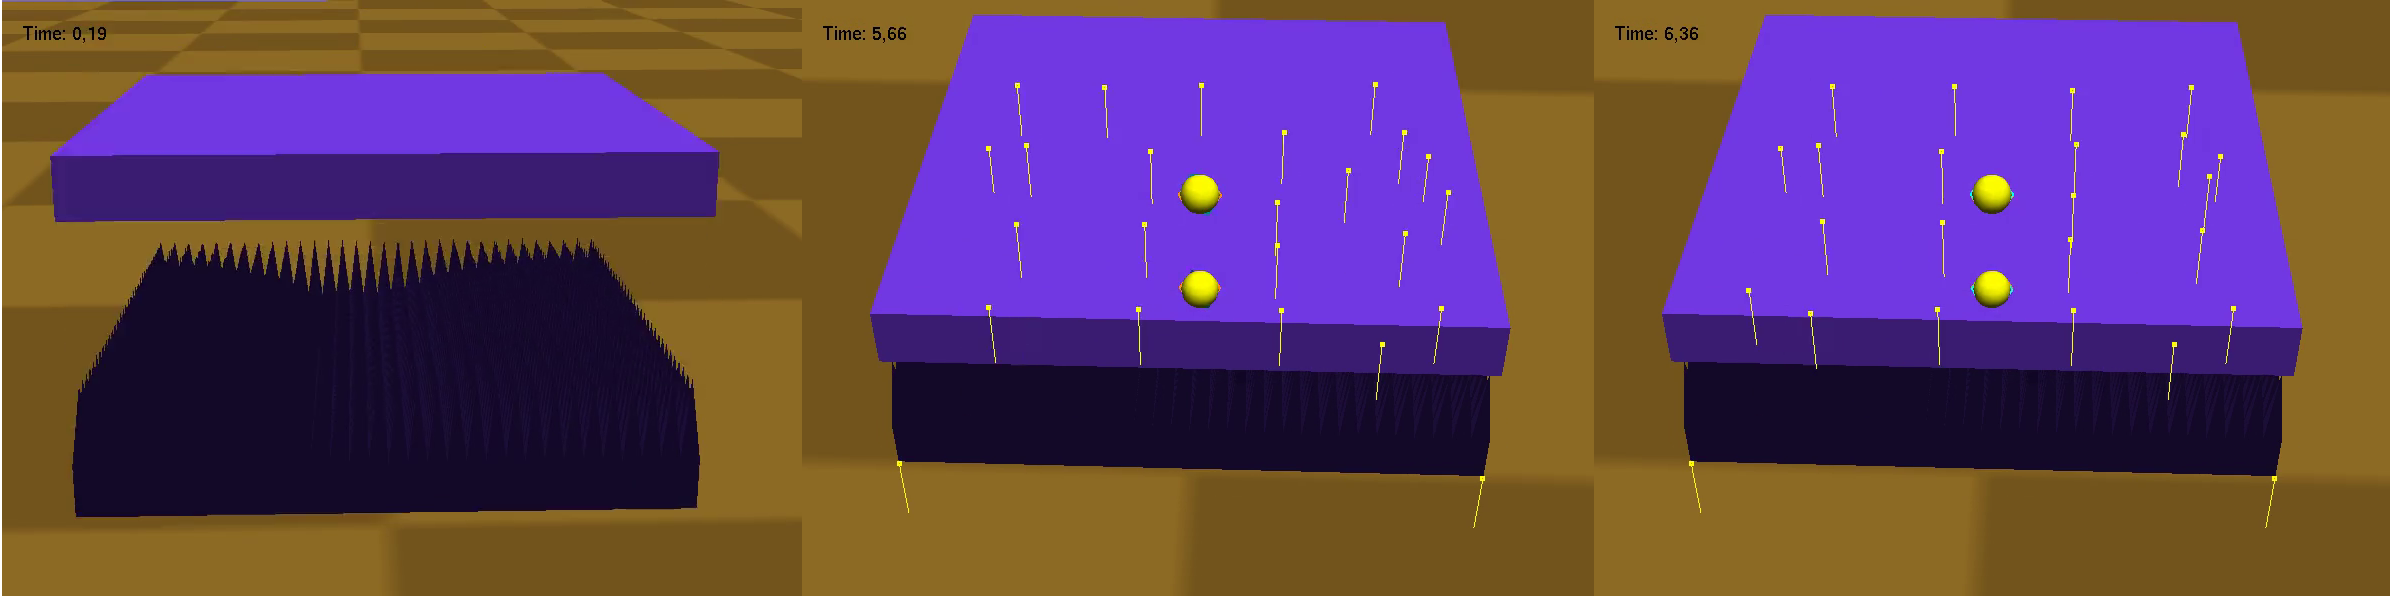
\includegraphics[width=0.95\columnwidth]     {images/ssoch/clustering}
        \caption{Illustrating two contact clustering methods on a 2,000-spike ``spiky block''. Left: hierarchical clustering.  Right: $k$-means clustering. Centers of pressure are draw}
        \label{fig:clustering}
        \end{center}
\end{figure}


\section{Contact stability metrics}

In the following section are introduced the metrics used in this work for evaluating the stability of contact points and contact forces at a fine granularity during the simulation of grasping.  These metrics correspond to the position, normal, and force dimensions of point contact models used in classical grasp analysis, which forms the basis of most grasp planning techniques.

\subsection{Contact Force Variation}

At equilibrium, we expect the contact forces exerted on the objects to be as close to constant as possible. Our first measurement penalizes fluctuations and spikes in force at an (ostensible) equilibrium state. 

The resultant contact force exerted on body $i$  is $f_i \equiv \int_{x\in S_i(q)} \rho_i(x) dx$, which the simulator approximates by a finite set of contact forces.  The contact force smoothness index measures the normalized standard deviation of resultant forces. (It may be possible to also include resultant torques  $m_i \equiv \int_{x\in S_i(q)} (x-o_i) \times \rho_i(x) dx$ but these are highly correlated to forces for most grasps so we ignore them.) 

Over a span of time $t$ where the object should be held in equilibrium by the physical hand, we measure the quantities $\sqrt{\|Var[f_i(t)]\|_F} / E[\|f_i(t)\|]$ for all bodies $i$ in the set $C$ of bodies touching the object.  Here $\|\cdot\|_F$ denotes the matrix Frobenius norm. We then report the final score (0 being best):
\begin{equation}
S_{cf} \equiv \frac{1}{|C|} \sum_{|i\in C|} \sqrt{\|Var[f_i(t)]\|_F} / E[||f_i(t)||].
\end{equation}

\subsection{Contact position and normal variation}
The second and third scores measure the stability of contact positions and normals during an equilibrium grasp.  A simulator generates a set of point contacts at location $x_1,\ldots,x_k$ and their corresponding normals $n_1,\ldots,n_k$ ($k$ varying by time step).  The scores measure the fluctuations of the average contact position $\hat{x}_i$ on body $i$ and average contact normal $\hat{n}_i$ over time (0 being best).

The equations are as follows:
\begin{equation}
S_{cp} \equiv \frac{1}{C} \sum_{|i\in C|} \sqrt{\|Var[\hat{x}_i(t)]\|_F}
\end{equation}
\begin{equation}
S_{cn} \equiv \frac{1}{C} \sum_{|i\in C|} \sqrt{\|Var[\hat{n}_i(t)]\|_F}
\end{equation}

An example of these results for the spiky plane example is given in Fig.~\ref{fig:SpikyStability}.

\begin{figure}
\centering
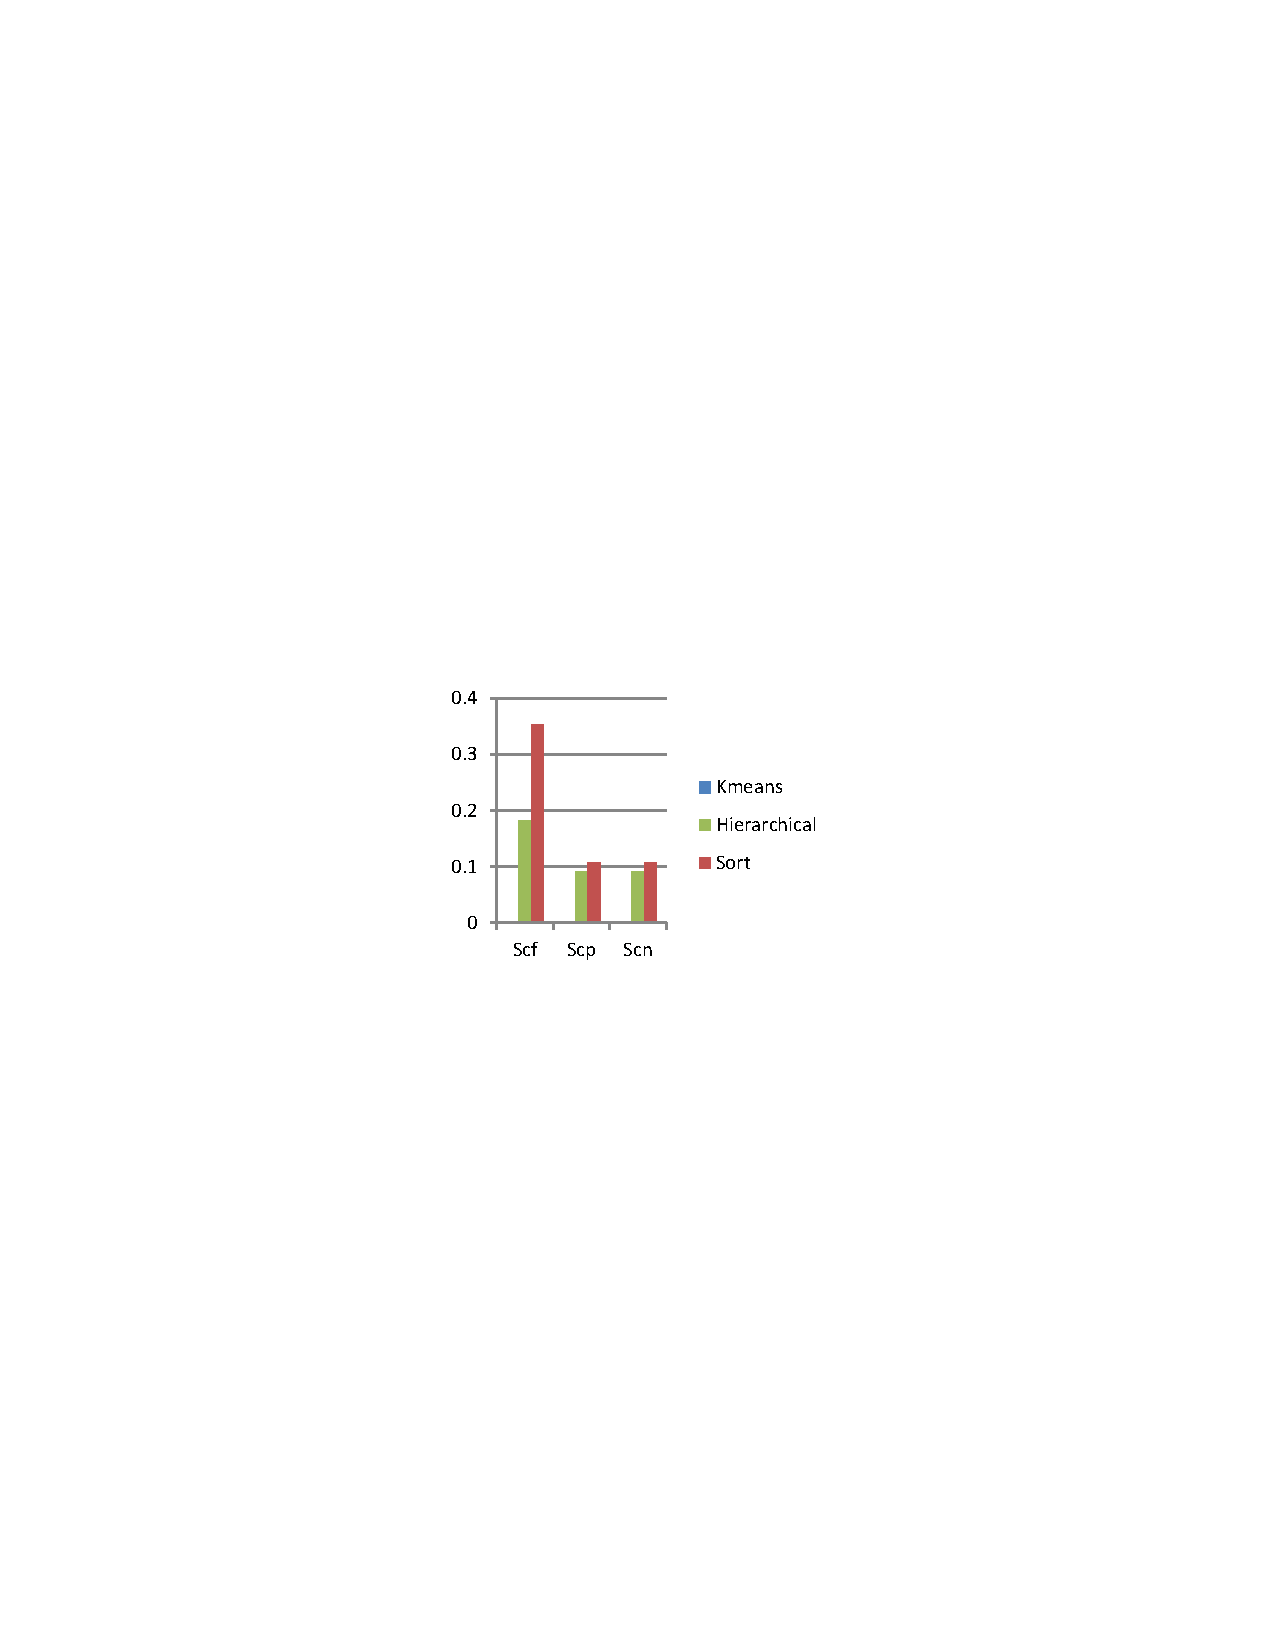
\includegraphics[width=0.6\columnwidth]{images/ssoch/spiky_metrics.pdf}
\caption{Contact stability metrics $S_{cf}$, $S_{cp}$, and $S_{cn}$ over the spiky plane example of Fig.~\ref{fig:clustering} for various clustering methods. K-means leads to almost imperceptible instability (~$1E-17$ for all three indices)}
\label{fig:SpikyStability}
\end{figure}


\subsection{Experiments}
\label{experiments5}

Experiments are performed both with a RightHand Robotics' ReFlex Hand and Pisa/IIT SoftHand.  A set of grasps with varying degrees of robustness are designed by human inspection and tested on a set of physical objects and their simulated counterparts.

\begin{table}[hbt]
   \begin{center}
   \begin{tabular}{| c | c | c |}
   \hline
   Object & Weight & Size \\
   \cline{1-3}
   Hammer					& 480 g   	& 290mmX35mmX95mm      \\\hline
   Spray Bottle (no cap)	& 703.5 g   & 220mmX120mmX40mm      \\\hline
   Spray Bottle (with cap)	& 726 g   	& 270mmX120mmX40mm      \\\hline
   Ketchup				& 948.6 g   & 195mmX100mmX70mm   \\\hline
   Pasta Box				& 487g      & 120mmX19mmX72mm      \\\hline
   \end{tabular}
   \end{center}
   \caption{Weight of all the objects and approximate dimensions}
   \label{table:object}
\end{table}


For the two hands, a series of grasps are selected for each object in the set:
\emph{hammer, ketchup bottle, spray bottle} and a \emph{pasta box}.
The \emph{hammer} and the \emph{pasta box} are modeled by hand. The rest of the objects have been scanned using a \emph{Makerbot Digitizer}. The results and details of the mesh reconstruction are shown and detailed in Fig. \ref{meshes}.
Dimensions are given in Tab.~\ref{table:object}.
We assume an approximate mass distribution for the \emph{hammer}, and for the mass of the the rest of the objects.
In all the experiments, the objects are laying on a table.


Human-chosen grasps are selected in order to have a selection of robust grasps, non-robust grasps, and failed grasps as described in Tab.~\ref{table:grasp}. Robust grasps tolerate small variations in the object pose and disturbance forces. Non-robust grasps succeed some of the time, but do not always tolerate such variations.  Failed grasps fail consistently.  

The hands and the table are marked with fiducial markers, and their position and orientation are recorded for each grasp via a Microsoft Kinect camera. The objects are placed on the table in a known pose, and the grasps illustrated in Fig. \ref{hammer}, \ref{heinz_bottle} and \ref{spray} are performed. For every nominal grasp pose, the hand has been positioned manually on the desired configuration via the gravity compensation control of the \emph{Baxter} robot. A set of $6$ trials is performed for each grasp, and grasp scores are averaged over the attempts over three indices:

\begin{table}[hbt]
   \begin{center}
   \begin{tabular}{| p{1.5cm}  | c | c | p{2.5cm} | c |}
   \hline
   Object   & Pose  & Effort &  Grasp Position  & Preshape \\
   \cline{1-5}
   Hammer					& P1   		&	0.3	& 	Handle	& 	0   \\\hline
   Hammer					& P2   		&	0.3	& 	CoG	& 	0   \\\hline
   Hammer					& P3   		&	0.3	& 	Head	& 	0.5 \\\hline
   Spray Bottle (no cap)	& P1   		&	0.2	&   Low (spray facing outside) 	&	0	\\\hline
   Spray Bottle (no cap)	& P2   		&	0.2	&   High  (spray facing outside)  	&	0	\\\hline
   Spray Bottle (no cap)	& P3   		&	0.2	&   Low (spray facing inside)  	&	0	\\\hline
   Spray Bottle (no cap)	& P4   		&	0.2	&   High (spray facing inside)    			&	0	\\\hline   
   Spray Bottle (with cap)	& P1   		&	0.2	&   High   	&	0	\\\hline
   %Ketchup				& P1   		&	0.3	&   Cap   	&	1.5	\\\hline %got experiment, but not simulation
   Ketchup				& P1   		&	0.3	&   Cap   	&	1.5	\\\hline
   Ketchup				& P2   		&	0.3	&   Under cap ridge   	&	1.3	\\\hline
   Ketchup				& P3   		&	0.2	&   Lateral ridge   	&	0	\\\hline
   Ketchup				& P4   		&	0.2	&   Above lateral ridge   	&	0	\\\hline
   Pasta Box				& P1   		&	N/A	&   Top, parallel   	&   N/A	\\\hline
   Pasta Box				& P2   		&	N/A	&   Top, tilt along yaw   	&	N/A \\\hline
   Pasta Box				& P3   		&	N/A	&   Side   	&   N/A	\\\hline   
   
   \end{tabular}
   \end{center}
   \caption{Grasp configuration}
   \label{table:grasp}
\end{table}


\begin{figure}[!hbt]
\begin{center}
        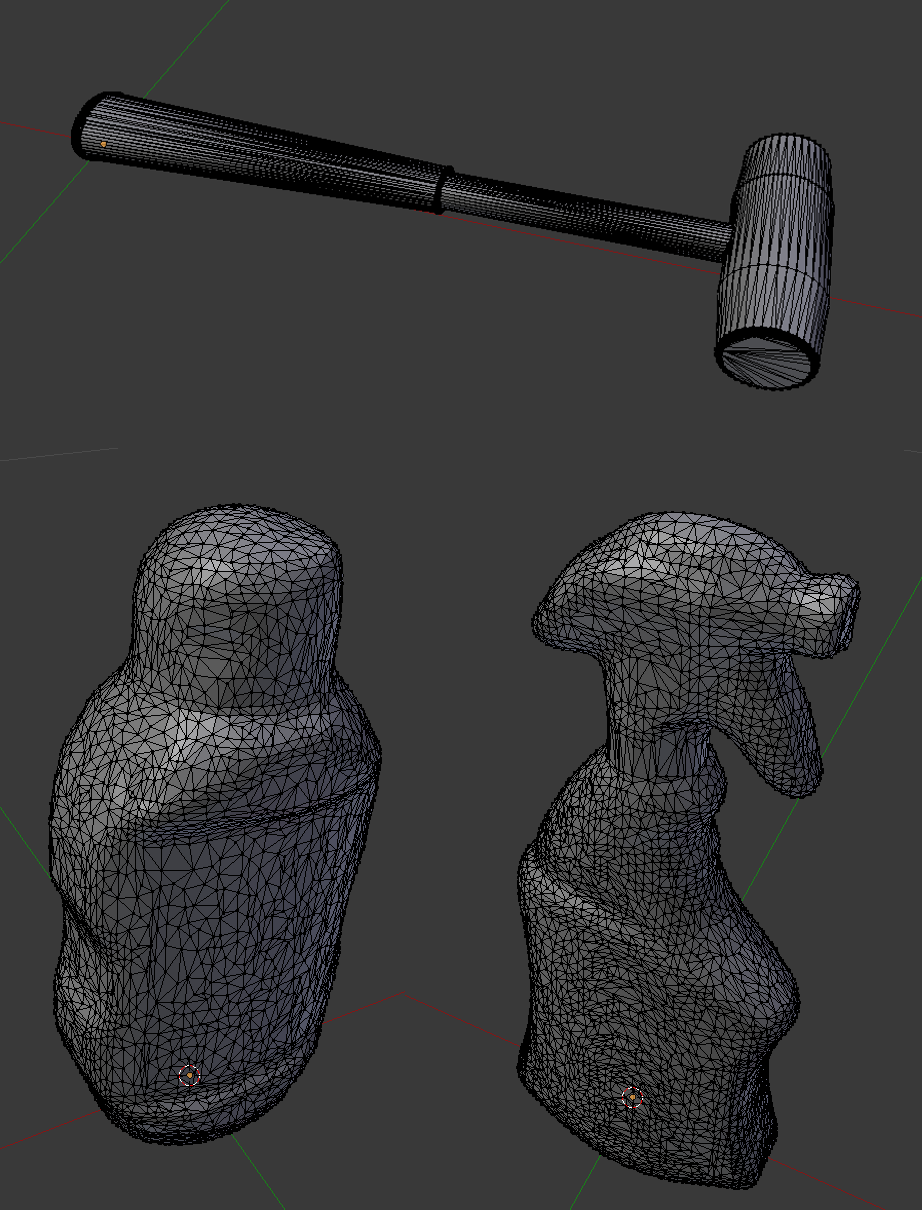
\includegraphics[width=0.6\columnwidth]     {images/ssoch/meshes}
        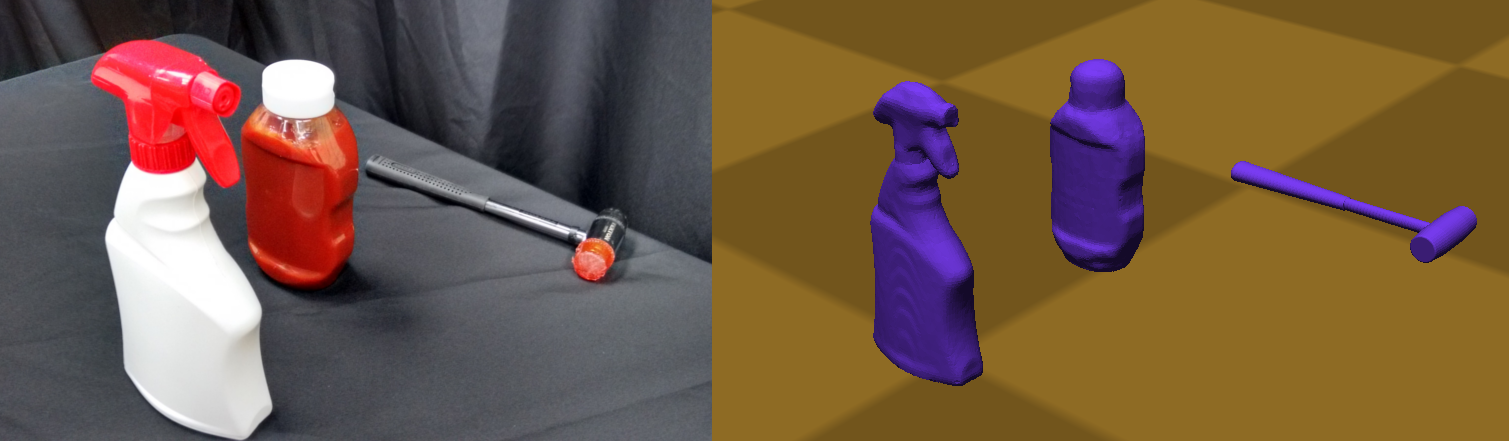
\includegraphics[width=0.95\columnwidth]     {images/ssoch/objects}
        \caption{The 3d laser range scans are reconstructed using Poisson surface reconstruction, and the number of faces of the mesh is then reduced using Quadric Edge Collapse Decimation. All the meshes have a number of faces between $8000$ and $12000$. As a last step, the bottom of the object is manually cropped to a flat surface.}
        \label{meshes}
        \end{center}
\end{figure}

\begin{figure}[!hbt]
\begin{center}
        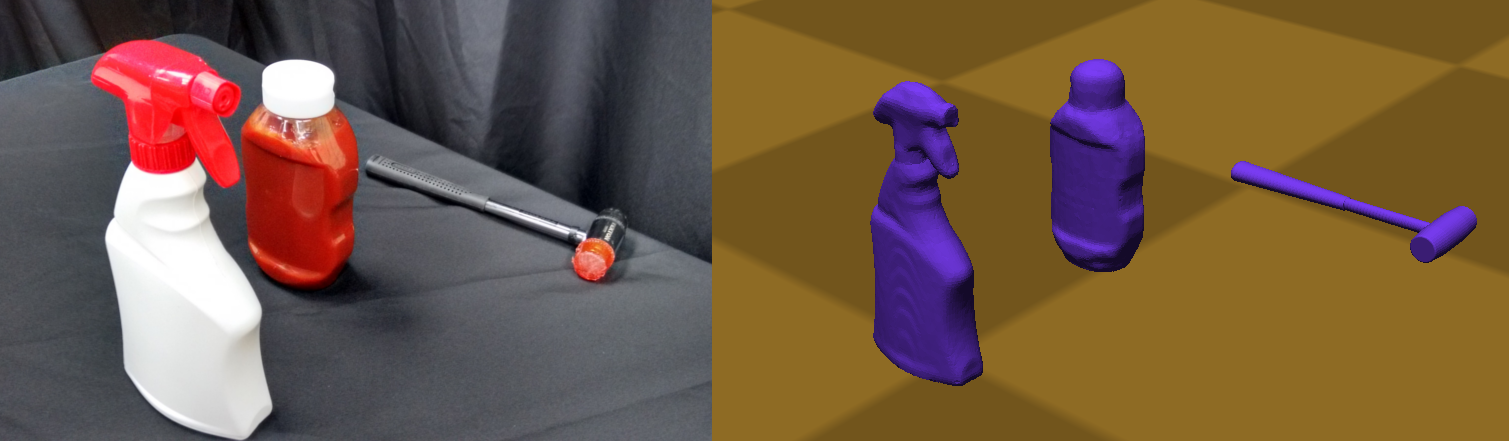
\includegraphics[width=0.95\columnwidth]     {images/ssoch/objects}
        \caption{comparison side by side of the real objects and the 3d scanned}
        \label{objects}
        \end{center}
\end{figure}



\begin{itemize}
\item \textbf{$S1$ object pose deviation}. This is designed in order to be performed easily by eye without complicated measurements attempts. As it can be seen in \ref{real_score} it is practically useful only in the \emph{hammer} set of grasps, because of the advantageous lever the CoM has on the grasp. In the bidimensional case, the index uniformly discretizes the possible swing angle of the hammer in $3$ regions, with scores $1$, $0.6$ and $0.3$. The score will be $0$ in case of an unsuccessful grasp.
\item \textbf{$S2$ the normalized number of fingers in contact}. For the Reflex Hand, the index can assume values $1$ for a three-fingers grasp and $0.5$ for a two fingers grasp. For the Soft Hand, the index can assume values $1$,$0.75$,$0.5$ and $0.25$.
\item \textbf{$S3$ ability to resist perturbation}. By applying a shaking motion on the hand of the robot, we check if one of the previous indices changes in value as a consequence of the perturbation, in which case the score will be $0.6$. In case of a dropped object as a consequence of the perturbation, the score will be $0.3$.
\end{itemize}


\begin{figure}[!hbt]
\begin{center}
        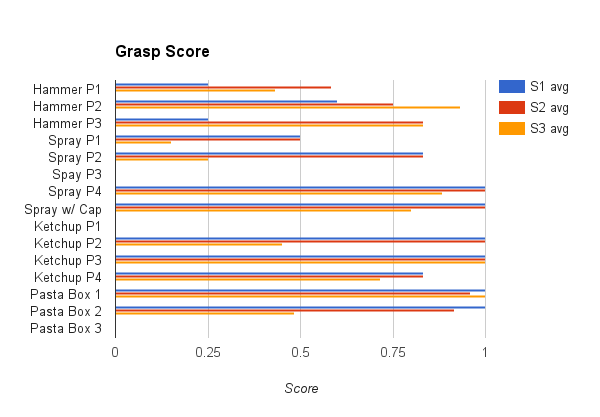
\includegraphics[width=0.95\columnwidth]     {images/ssoch/real_score}
        \caption{Grasp scores for physical experiments. On the \emph{x} axis, $1-3$ are for \emph{hammer-P1} to \emph{hammer-P3}, $4-7$ are for \emph{spray-P1} to \emph{spray-P4}, while score $8$ is for \emph{spray-full-P1}, $9-13$ are for \emph{Ketchup-P1} to \emph{Ketchup-P5}}
        \label{real_score}
        \end{center}
\end{figure}

The grasp procedure for the \emph{Reflex Hand} consists in simultaneously closing each finger until the motor's effort threshold is met, at which point the finger is stopped. For the \emph{Soft Hand}, the fingers close simultaneously until the nominal torque limit of the single actuator is reached. To check if the grasp is successful, the object is then raised. If successfully raised, the robustness of the grasp is checked by shaking the gripper by hand.


\begin{figure}[!hbt]
\begin{center}
        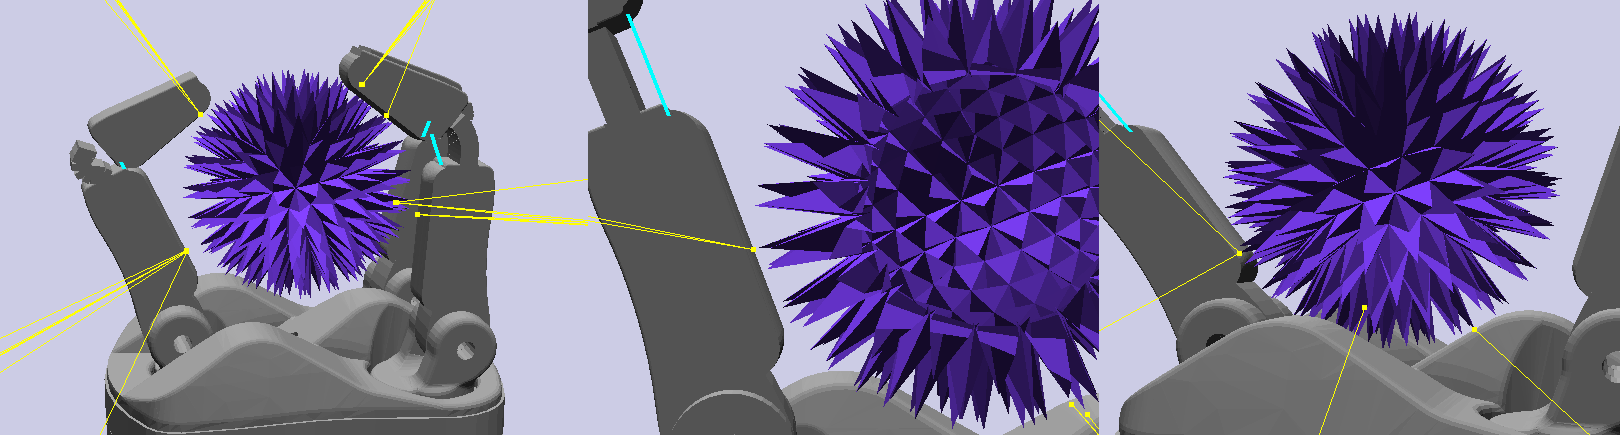
\includegraphics[width=0.95\columnwidth]     {images/ssoch/preshrink}
        \caption{Since the \emph{BLEM} method works by expanding the meshes via Minkowski dilation, a preshrink method was introduced so that the boundary layer added to a preshrunk mesh will sum up to the approximate size of the original mesh. In figure, from left to right, a $5mm$ boundary layer shows gaps between the hand and the object, a $1mm$ boundary layer, and a $1mm$ layer with preshrink. }
        \label{Preshrink}
        \end{center}
\end{figure}


The grasp is then performed in simulation.
We simulate the \emph{Reflex Hand} using \emph{Klamp't} v$0.6.2$, and the \emph{Soft Hand} using \emph{Gazebo} v$4.0$ with a preliminary version of the \emph{Soft Hand plugin}~\cite{Rosales15SHP}.
The \emph{Gazebo} simulator is tested against our patch \cite{Rocchi15GBP} where \emph{BLEM} is used. In Gazebo, the simple contact sorting algorithm is used for contact filtering. The \emph{Klamp't} simulator is tested with  \emph{BLEM} against the default in Open Dynamics Engine \emph{OPCODE}.  In Klamp't examples, we use $k$-means clustering with a maximum of 20 contacts.

The robot's motor parameters, tendon Baumgarte stability constants, and friction parameters were tuned by hand so that the hands would move qualitatively similarly to the real hands, and to be stable both in free space motion and while grasping on a spherical object.  No quantitative calibration procedure was performed.



\begin{figure*}[!!hbt]
\begin{center}
{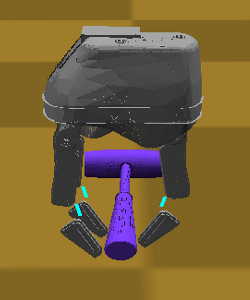
\includegraphics[width=0.225\columnwidth]     {images/ssoch/fig/hammer_P1}\label{hammer_P1}}%
{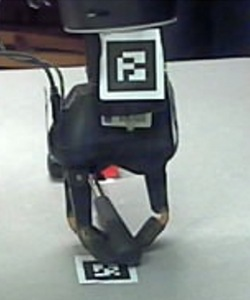
\includegraphics[width=0.225\columnwidth]     {images/ssoch/fig/hammer_p1_1}\label{hammer_p1_1}}
{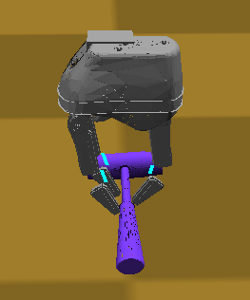
\includegraphics[width=0.225\columnwidth]     {images/ssoch/fig/hammer_P2}\label{hammer_P2}}%
{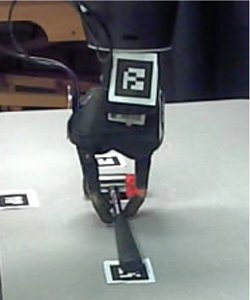
\includegraphics[width=0.225\columnwidth]     {images/ssoch/fig/hammer_p2_1}\label{hammer_p2_1}}
{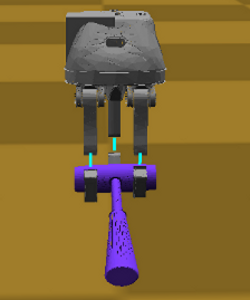
\includegraphics[width=0.225\columnwidth]     {images/ssoch/fig/hammer_P3}\label{hammer_P3}}%
{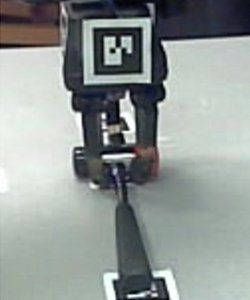
\includegraphics[width=0.225\columnwidth]     {images/ssoch/fig/hammer_p3_1}\label{hammer_p3_1}}
        \caption{Comparison between simulation and experiment: \emph{Hammer-P1}, \emph{Hammer-P2}, \emph{Hammer-P3}}
        \label{hammer}
        \end{center}
\end{figure*}


\begin{figure*}[!!hbt]
\begin{center}
{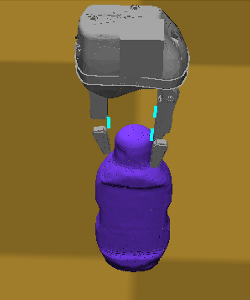
\includegraphics[width=0.11\textwidth]     {images/ssoch/fig/heinz_P1}\label{heinz_P1}}%
{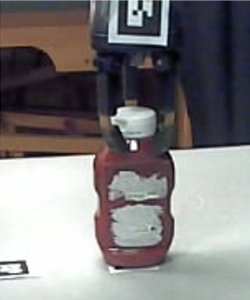
\includegraphics[width=0.11\textwidth]    {images/ssoch/fig/heinz_p1_1}\label{heinz_p1_1}}
{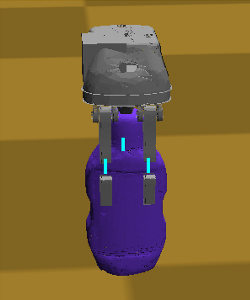
\includegraphics[width=0.11\textwidth]{images/ssoch/fig/heinz_P2}\label{heinz_P2}}%
{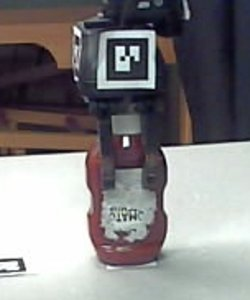
\includegraphics[width=0.11\textwidth]{images/ssoch/fig/heinz_p2_1}\label{heinz_p2_1}}
%{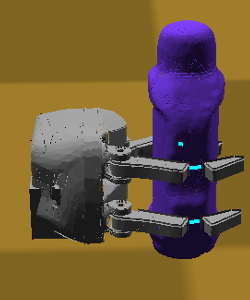
\includegraphics[width=0.09\textwidth]{images/ssoch/fig/heinz_P3}\label{heinz_P3}}%
%{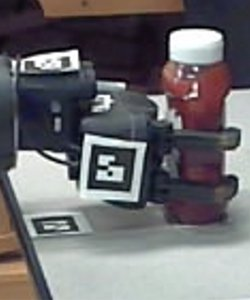
\includegraphics[width=0.09\textwidth]    {images/ssoch/fig/heinz_p3_1}\label{heinz_p3_1}}
{ 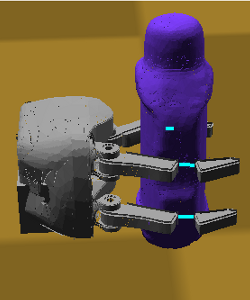
\includegraphics[width=0.11\textwidth]     {images/ssoch/fig/heinz_P4}\label{heinz_P4}}%
{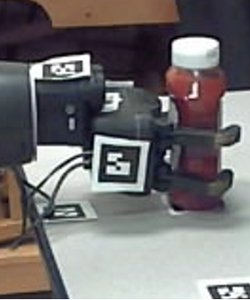
\includegraphics[width=0.11\textwidth]{images/ssoch/fig/heinz_p4_1}\label{heinz_p4_1}}
{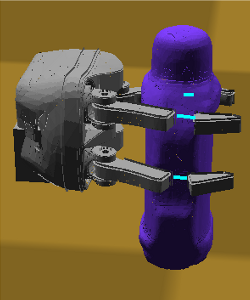
\includegraphics[width=0.11\textwidth]{images/ssoch/fig/heinz_P5}\label{heinz_P5}}%
{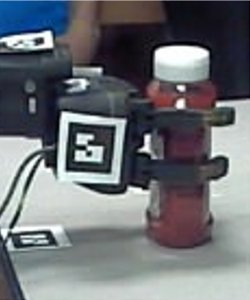
\includegraphics[width=0.11\textwidth]{images/ssoch/fig/heinz_p5_1}\label{heinz_p5_1}}
        \caption{Comparison between simulation and experiment: \emph{Ketchup-P1}, \emph{Ketchup-P2}, \emph{Ketchup-P3}, \emph{Ketchup-P4}}
        \label{heinz_bottle}
        \end{center}
\end{figure*}


\begin{figure*}[!!hbt]
\begin{center}
{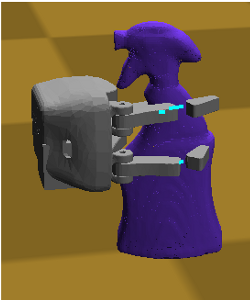
\includegraphics[width=0.09\textwidth]     {images/ssoch/fig/spray_full_P1}\label{spray_full_P1}}%
{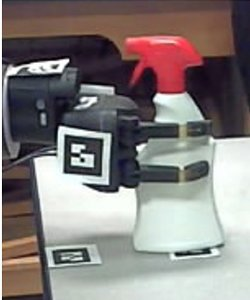
\includegraphics[width=0.09\textwidth]     {images/ssoch/fig/spray_full_p1}\label{spray_full_p1}}
{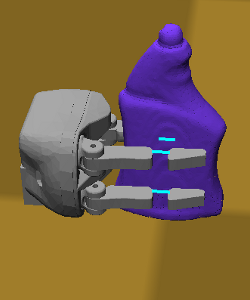
\includegraphics[width=0.09\textwidth]{images/ssoch/fig/spray_P1}\label{spray_P1}}%
{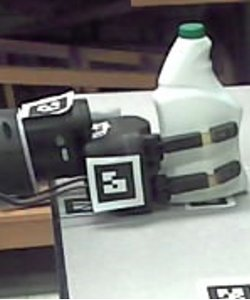
\includegraphics[width=0.09\textwidth]{images/ssoch/fig/spray_p1}\label{spray_p1}}
{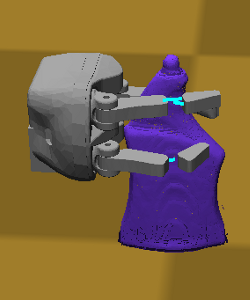
\includegraphics[width=0.09\textwidth]{images/ssoch/fig/spray_P2}\label{spray_P2}}%
{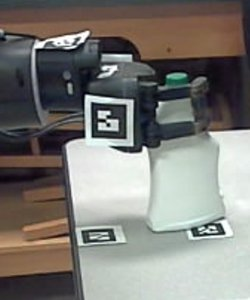
\includegraphics[width=0.09\textwidth]{images/ssoch/fig/spray_p2}\label{spray_p2}}
{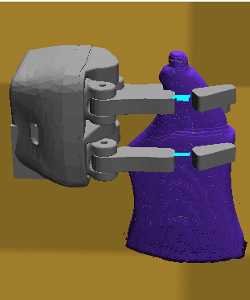
\includegraphics[width=0.09\textwidth]{images/ssoch/fig/spray_P3}\label{spray_P3}}%
{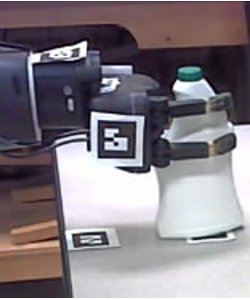
\includegraphics[width=0.09\textwidth]{images/ssoch/fig/spray_p3}\label{spray_p3}}
{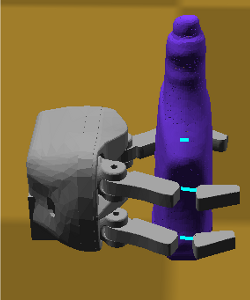
\includegraphics[width=0.09\textwidth]{images/ssoch/fig/spray_P4}\label{spray_P4}}%
{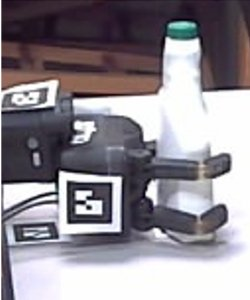
\includegraphics[width=0.09\textwidth]{images/ssoch/fig/spray_p4}\label{spray_p4}}
        \caption{Comparison between simulation and experiment: \emph{Spray Bottle (with cap)}, \emph{Spray Bottle (no cap) - P1}, \emph{Spray Bottle (no cap) - P2}, \emph{Spray Bottle (no cap) - P3}, \emph{Spray Bottle (no cap) - P4}}
        \label{spray}
        \end{center}
\end{figure*}


\begin{figure*}[!!hbt]
\begin{center}
{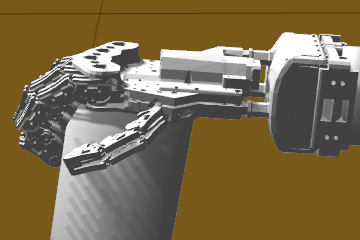
\includegraphics[height=0.24\columnwidth]     {images/ssoch/fig/kh_changes/softhand_p1_simu01}}%
{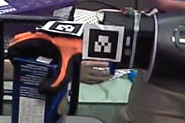
\includegraphics[height=0.24\columnwidth]     {images/ssoch/fig/kh_changes/softhand_p1_grasp}}
{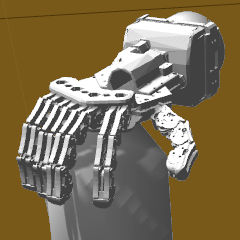
\includegraphics[height=0.24\columnwidth]     {images/ssoch/fig/kh_changes/softhand_p2_simu01}}%
{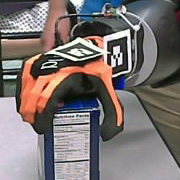
\includegraphics[height=0.24\columnwidth]     {images/ssoch/fig/kh_changes/softhand_p2_grasp}}
{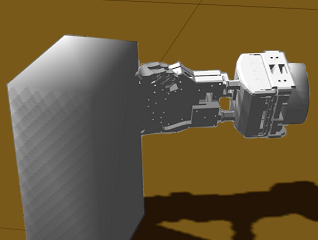
\includegraphics[height=0.24\columnwidth]     {images/ssoch/fig/kh_changes/softhand_p3_simu01}}%
{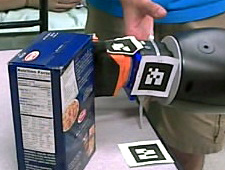
\includegraphics[height=0.24\columnwidth]     {images/ssoch/fig/kh_changes/softhand_p3_grasp}}
        \caption{Comparison between simulation and experiment: {\em Pasta Box - P1}, {\em Pasta Box - P2}, and {\em Pasta Box - P3}.}
        \label{pasta_box}
        \end{center}
\end{figure*}


The simulation procedure is as follows:
\begin{itemize}
\item The object and hands are spawned in the pregrasp and preshape configuration,
\item As in the physical hardware, the hands are closed until an actuator force threshold is reached.
\item The hand is lifted by 10cm,
\item The grasp is perturbed by commanding jerking movements of the wrist,
\item Finally the hand opens to drop the object.
\end{itemize}

\begin{figure*}
\centering
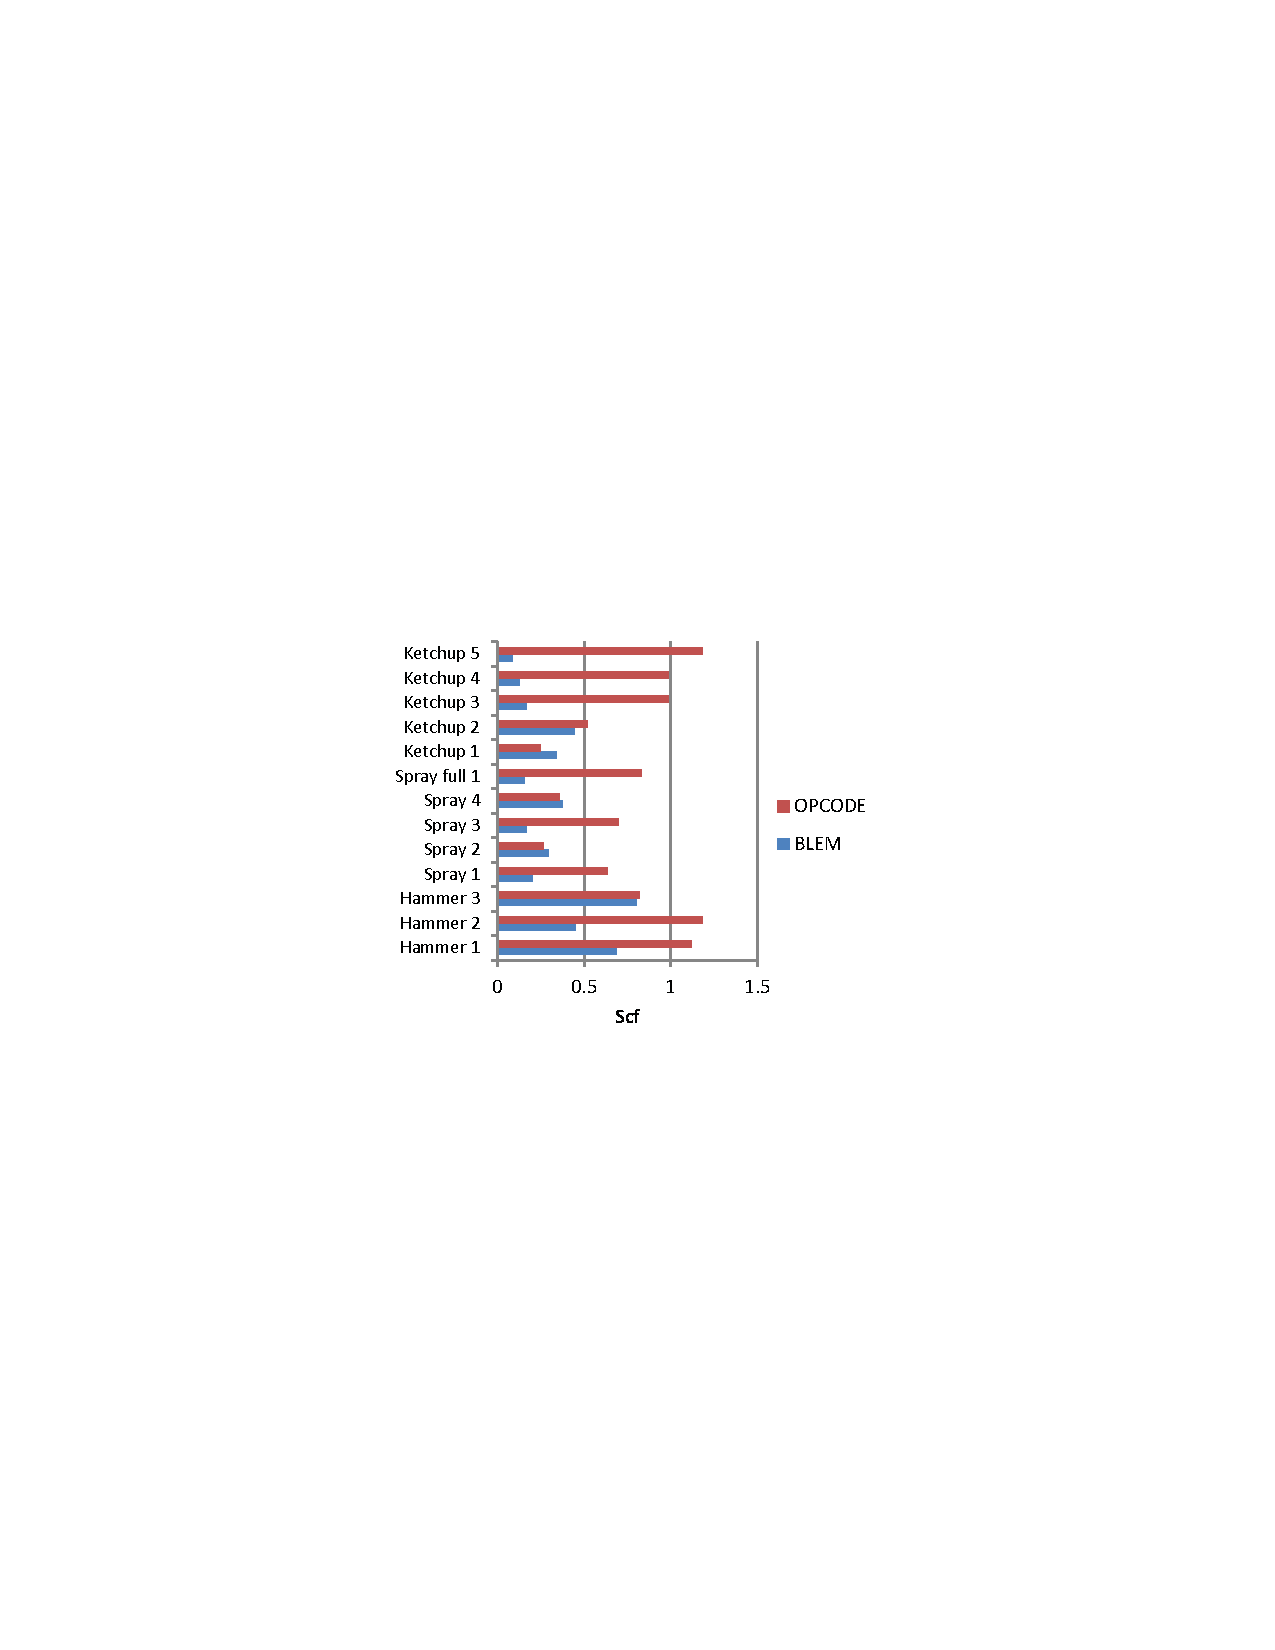
\includegraphics[width=0.32\textwidth]{images/ssoch/scf_metrics.pdf}
\includegraphics[width=0.32\textwidth]{images/ssoch/scp_metrics.pdf}
\includegraphics[width=0.32\textwidth]{images/ssoch/scn_metrics.pdf}
\caption{Metrics $S_{cf}$, $S_{cp}$, and $S_{cn}$ over the simulated grasp set. Lower numbers are better.}
\label{fig:AllMetrics}
\end{figure*}

Fig.~\ref{fig:AllMetrics} illustrates the results of the contact stability indices between BLEM and OPCODE contact generation. It can be observed BLEM leads to higher stability in general, most strikingly for the contact normal metric.

\begin{table}[hbt]
   \begin{center}
   \begin{tabular}{| c | c  c | c c |}
   \hline
   Grasp & Grasped & Dropped & Grasped & Dropped\\
   \hline
    {\bf ReFlex} & \multicolumn{2}{c|}{{\bf ODE / BLEM}} & \multicolumn{2}{c|}{{\bf ODE / OPCODE}} \\
   \cline{1-5}
   Hammer 1	    & Y & Y & Y & {\bf N} \\
   Hammer 2	    & Y & Y & Y & Y \\
   Hammer 3	    & Y & Y & Y & {\bf N} \\
   ~Spray 1+	& Y & Y & Y & {\bf N} \\
   ~Spray 2+	& Y & Y & Y & {\bf N} \\
   ~Spray 3*	& Y & Y & Y & Y \\
   Spray 4	& Y & Y & Y & {\bf N} \\
   Spray Full 1	& Y & Y & Y & Y \\
   ~Ketchup 1*	& Y & Y & {\bf N} & -- \\
   Ketchup 2	& Y & Y & {\bf N} & -- \\
   Ketchup 3	& Y & Y & Y & {\bf N} \\
   Ketchup 4	& Y & Y & Y & {\bf N} \\
   \hline
   {\bf SoftHand} & \multicolumn{2}{c|}{{\bf Gazebo / BLEM}} & \multicolumn{2}{c|}{{\bf Gazebo / OPCODE}} \\
   \hline
   Pasta Box 1  & Y & Y & X & Y \\
   Pasta Box 2+ & Y & Y & X & Y \\
   Pasta Box 3* & N & -- & N  & -- \\
   \hline
   \end{tabular}
   \end{center}
   \caption{Success rates of ReFlex grasps (top) and SoftHand grasps (bottom) in simulation.  Asterisks indicate failed grasps on physical experiments. The plus sign indicates non robust grasps on physical experiments.  An entry of X  indicates variability for the same initial conditions.}
   \label{table:GraspSuccess}
\end{table}

Tab.~\ref{table:GraspSuccess} illustrates the results of simulations. 12/12 successful grasps were reliably grasped by BLEM and 9/12 were grasped by OPCODE. In all successful grasps, the object was securely held through perturbations.  In the two ODE/OPCODE failure cases, the hand  penetrated completely through the object without contact.  In the two Gazebo/OPCODE unreliable grasp cases, we observed  nondeterminism in the simulator which caused the grasp to fail in approximately 1/3 of simulation trials, even with the exact same initial conditions.

Perhaps more worrisome is the result that ODE/OPCODE did not successfully release the grasped object in 7/9 successful grasps.  This is explained by major interpenetration artifacts, in which the object gets ``stuck'' on the robot's finger and cannot be let go (Fig.~\ref{fig:OPCODEArtifact}. 

\begin{figure}
    \centering
    \includegraphics[width=0.25\textwidth]{opcode-artifact.png}
    \caption{An artifact exhibited in OPCODE causing the object to penetrate and then ``stick'' to the robot's finger.}
    \label{fig:OPCODEArtifact}
\end{figure}

BLEM did not successfully predict 2/3 failed grasps. This likely indicates an improperly calibrated coefficient of friction or absolute grasp force.  This suggests that although stable simulation is crucial for obtaining reasonable predictions, it is still challenging for simulation to accurately discern the boundary of feasible/infeasible grasps without considerable tuning.   An interesting area for future work would be to automatically tune the robot model to obtain a match with physical experiments.

Lastly, computation times during grasp for the \emph{Klamp't} case were similar between BLEM, with $~2.7$ms and OPCODE, with $\sim2.9$ms for each millisecond of simulated time. For Gazebo, the experimental BLEM patch resulted in computation times of $\sim2.4$ms against $\sim1.6$ms of OPCODE for each millisecond of simulated time. All measurements were taken on an Intel Core i5-4460 CPU @3.2HGz.

\subsection{Conclusions}
A series of simulation stability and fidelity criterion have been established. They have been tested on two different compliant and underactuated hardware platforms, the \emph{RightHand Robotics' Reflex Hand} and the \emph{Pisa/IIT SoftHand}. A set of grasps has been performed on the physical hardware using $4$ different objects of different shapes and characteristics, in different grasping scenarios, and then validated using \emph{Klamp't} and \emph{Gazebo}, using different techniques for \emph{contact clustering} and \emph{contact generation}. The experimental results show that  simulations performed with the \emph{BLEM} \emph{contact generation} algorithm and the \emph{k-means clustering} contact filtering algorithm have the highest stability indices, and also exhibit the fewest artifacts.
